\documentclass[]{book}
\usepackage{lmodern}
\usepackage{amssymb,amsmath}
\usepackage{ifxetex,ifluatex}
\usepackage{fixltx2e} % provides \textsubscript
\ifnum 0\ifxetex 1\fi\ifluatex 1\fi=0 % if pdftex
  \usepackage[T1]{fontenc}
  \usepackage[utf8]{inputenc}
\else % if luatex or xelatex
  \ifxetex
    \usepackage{mathspec}
  \else
    \usepackage{fontspec}
  \fi
  \defaultfontfeatures{Ligatures=TeX,Scale=MatchLowercase}
\fi
% use upquote if available, for straight quotes in verbatim environments
\IfFileExists{upquote.sty}{\usepackage{upquote}}{}
% use microtype if available
\IfFileExists{microtype.sty}{%
\usepackage{microtype}
\UseMicrotypeSet[protrusion]{basicmath} % disable protrusion for tt fonts
}{}
\usepackage[margin=1in]{geometry}
\usepackage{hyperref}
\hypersetup{unicode=true,
            pdftitle={R que R},
            pdfauthor={Enric Escorsa O'Callaghan},
            pdfborder={0 0 0},
            breaklinks=true}
\urlstyle{same}  % don't use monospace font for urls
\usepackage{natbib}
\bibliographystyle{apalike}
\usepackage{color}
\usepackage{fancyvrb}
\newcommand{\VerbBar}{|}
\newcommand{\VERB}{\Verb[commandchars=\\\{\}]}
\DefineVerbatimEnvironment{Highlighting}{Verbatim}{commandchars=\\\{\}}
% Add ',fontsize=\small' for more characters per line
\usepackage{framed}
\definecolor{shadecolor}{RGB}{248,248,248}
\newenvironment{Shaded}{\begin{snugshade}}{\end{snugshade}}
\newcommand{\AlertTok}[1]{\textcolor[rgb]{0.94,0.16,0.16}{#1}}
\newcommand{\AnnotationTok}[1]{\textcolor[rgb]{0.56,0.35,0.01}{\textbf{\textit{#1}}}}
\newcommand{\AttributeTok}[1]{\textcolor[rgb]{0.77,0.63,0.00}{#1}}
\newcommand{\BaseNTok}[1]{\textcolor[rgb]{0.00,0.00,0.81}{#1}}
\newcommand{\BuiltInTok}[1]{#1}
\newcommand{\CharTok}[1]{\textcolor[rgb]{0.31,0.60,0.02}{#1}}
\newcommand{\CommentTok}[1]{\textcolor[rgb]{0.56,0.35,0.01}{\textit{#1}}}
\newcommand{\CommentVarTok}[1]{\textcolor[rgb]{0.56,0.35,0.01}{\textbf{\textit{#1}}}}
\newcommand{\ConstantTok}[1]{\textcolor[rgb]{0.00,0.00,0.00}{#1}}
\newcommand{\ControlFlowTok}[1]{\textcolor[rgb]{0.13,0.29,0.53}{\textbf{#1}}}
\newcommand{\DataTypeTok}[1]{\textcolor[rgb]{0.13,0.29,0.53}{#1}}
\newcommand{\DecValTok}[1]{\textcolor[rgb]{0.00,0.00,0.81}{#1}}
\newcommand{\DocumentationTok}[1]{\textcolor[rgb]{0.56,0.35,0.01}{\textbf{\textit{#1}}}}
\newcommand{\ErrorTok}[1]{\textcolor[rgb]{0.64,0.00,0.00}{\textbf{#1}}}
\newcommand{\ExtensionTok}[1]{#1}
\newcommand{\FloatTok}[1]{\textcolor[rgb]{0.00,0.00,0.81}{#1}}
\newcommand{\FunctionTok}[1]{\textcolor[rgb]{0.00,0.00,0.00}{#1}}
\newcommand{\ImportTok}[1]{#1}
\newcommand{\InformationTok}[1]{\textcolor[rgb]{0.56,0.35,0.01}{\textbf{\textit{#1}}}}
\newcommand{\KeywordTok}[1]{\textcolor[rgb]{0.13,0.29,0.53}{\textbf{#1}}}
\newcommand{\NormalTok}[1]{#1}
\newcommand{\OperatorTok}[1]{\textcolor[rgb]{0.81,0.36,0.00}{\textbf{#1}}}
\newcommand{\OtherTok}[1]{\textcolor[rgb]{0.56,0.35,0.01}{#1}}
\newcommand{\PreprocessorTok}[1]{\textcolor[rgb]{0.56,0.35,0.01}{\textit{#1}}}
\newcommand{\RegionMarkerTok}[1]{#1}
\newcommand{\SpecialCharTok}[1]{\textcolor[rgb]{0.00,0.00,0.00}{#1}}
\newcommand{\SpecialStringTok}[1]{\textcolor[rgb]{0.31,0.60,0.02}{#1}}
\newcommand{\StringTok}[1]{\textcolor[rgb]{0.31,0.60,0.02}{#1}}
\newcommand{\VariableTok}[1]{\textcolor[rgb]{0.00,0.00,0.00}{#1}}
\newcommand{\VerbatimStringTok}[1]{\textcolor[rgb]{0.31,0.60,0.02}{#1}}
\newcommand{\WarningTok}[1]{\textcolor[rgb]{0.56,0.35,0.01}{\textbf{\textit{#1}}}}
\usepackage{longtable,booktabs}
\usepackage{graphicx,grffile}
\makeatletter
\def\maxwidth{\ifdim\Gin@nat@width>\linewidth\linewidth\else\Gin@nat@width\fi}
\def\maxheight{\ifdim\Gin@nat@height>\textheight\textheight\else\Gin@nat@height\fi}
\makeatother
% Scale images if necessary, so that they will not overflow the page
% margins by default, and it is still possible to overwrite the defaults
% using explicit options in \includegraphics[width, height, ...]{}
\setkeys{Gin}{width=\maxwidth,height=\maxheight,keepaspectratio}
\IfFileExists{parskip.sty}{%
\usepackage{parskip}
}{% else
\setlength{\parindent}{0pt}
\setlength{\parskip}{6pt plus 2pt minus 1pt}
}
\setlength{\emergencystretch}{3em}  % prevent overfull lines
\providecommand{\tightlist}{%
  \setlength{\itemsep}{0pt}\setlength{\parskip}{0pt}}
\setcounter{secnumdepth}{5}
% Redefines (sub)paragraphs to behave more like sections
\ifx\paragraph\undefined\else
\let\oldparagraph\paragraph
\renewcommand{\paragraph}[1]{\oldparagraph{#1}\mbox{}}
\fi
\ifx\subparagraph\undefined\else
\let\oldsubparagraph\subparagraph
\renewcommand{\subparagraph}[1]{\oldsubparagraph{#1}\mbox{}}
\fi

%%% Use protect on footnotes to avoid problems with footnotes in titles
\let\rmarkdownfootnote\footnote%
\def\footnote{\protect\rmarkdownfootnote}

%%% Change title format to be more compact
\usepackage{titling}

% Create subtitle command for use in maketitle
\newcommand{\subtitle}[1]{
  \posttitle{
    \begin{center}\large#1\end{center}
    }
}

\setlength{\droptitle}{-2em}
  \title{R que R}
  \pretitle{\vspace{\droptitle}\centering\huge}
  \posttitle{\par}
  \author{Enric Escorsa O'Callaghan}
  \preauthor{\centering\large\emph}
  \postauthor{\par}
  \predate{\centering\large\emph}
  \postdate{\par}
  \date{1/4/2017}

\usepackage{booktabs}
\usepackage{amsthm}
\makeatletter
\def\thm@space@setup{%
  \thm@preskip=8pt plus 2pt minus 4pt
  \thm@postskip=\thm@preskip
}
\makeatother

\usepackage{amsthm}
\newtheorem{theorem}{Theorem}[chapter]
\newtheorem{lemma}{Lemma}[chapter]
\theoremstyle{definition}
\newtheorem{definition}{Definition}[chapter]
\newtheorem{corollary}{Corollary}[chapter]
\newtheorem{proposition}{Proposition}[chapter]
\theoremstyle{definition}
\newtheorem{example}{Example}[chapter]
\theoremstyle{definition}
\newtheorem{exercise}{Exercise}[chapter]
\theoremstyle{remark}
\newtheorem*{remark}{Remark}
\newtheorem*{solution}{Solution}
\begin{document}
\maketitle

{
\setcounter{tocdepth}{1}
\tableofcontents
}

\includegraphics[width=2.78in]{fotoenric2}

Este trabajo de \emph{Enric Escorsa O'Callaghan} se ofrece bajo Licencia
\href{https://creativecommons.org/licenses/by-nc-sa/4.0/es/}{Creative
Commons Reconocimiento-NoComercial-CompartirIgual 4.0 España (CC
BY-NC-SA 4.0 ES)} cuyo texto legal está disponible en
\url{https://creativecommons.org/licenses/by-nc-sa/4.0/es}


\includegraphics[width=1.22in]{cc}

\hypertarget{prefacio}{%
\chapter{Prefacio}\label{prefacio}}

\begin{quote}
``Trabajando sobre los datos inmediatos de la realidad, nuestra
consciencia elabora el universo en el que vivimos realmente''

--- Aldous Huxley
\end{quote}

Este libro es una introducción muy básica y breve en español al lenguaje
de programación estadística \textbf{R}. Está dirigido a no programadores
(con ánimo de que empiecen a serlo un poquito cuando lo hayan leído).

R permite obtener todo tipo de datos (estructurados, no estructurados,
numéricos, textuales, etc.) de dondequiera que estén (bases de datos,
tablas, páginas web, etc.) y aplicarles tratamientos y métricas
estadísticas, así como generar todo tipo de visualizaciones que nos
ayuden a describirlos y entenderlos mejor; pero también automatizar
estos procesos, integrando distintas funciones, llegando a generar
modelos para, por ejemplo, detectar patrones y asociaciones interesantes
que estaban escondidas o hasta lograr predecir que ocurrirá, en base a
determinadas tendencias.

Todo ello, se puede hacer en R de una forma ágil, amigable, gratuita,
fresca y no encorsetada, en el contexto de una enorme y dinámica
comunidad global de usuarios que favorece la colaboración y el
aprendizaje continuo, la usabilidad y reproducibilidad de los resultados
que se generan y la incorporación de los últimos avances científicos en
análisis de datos y aprendizaje automático (\emph{Machine Learning}).

Este libro se escribió usando R -sí, ¡con R también podrás escribir
libros!- mediante el método de escritura \textbf{Markdown}, que permite
ir creando los contenidos sin preocuparte demasiado del formato final y
luego exportar fácilmente a los formatos deseados (por ejemplo: PDF,
ePub, HTML para publicarlo en una web, etc.)

Si quisieras escribir un libro como este desde R, lo puedes hacer
instalándote el paquete \textbf{bookdown} \citep{R-bookdown}. Ya
hablaremos de qué son los paquetes - \emph{packages} en inglés- y que
nos permiten; empecemos.

\hypertarget{indice-de-contenidos}{%
\section{Indice de contenidos}\label{indice-de-contenidos}}

El libro se estructura en los siguientes capítulos (si estás leyendo la
versión web del libro a la izquierda de la pantalla -o desplegándola
desde arriba- verás una barra de navegación que puedes usar para para
avanzar en los contenidos):

\begin{itemize}
\item
  Capítulo \ref{prefacio}: \textbf{Prefacio}
\item
  Capítulo \ref{intro}: \textbf{Introducción a R}
\item
  Capítulo \ref{r-para-explorar}: \textbf{R para explorar}
\item
  Capítulo \ref{r-para-predecir}: \textbf{R para predecir}
\item
  Capítulo \ref{r-para-visualizar}: \textbf{R para visualizar}
\item
  Capítulo \ref{r-que-r}: \textbf{R que R}
\end{itemize}

\hypertarget{intro}{%
\chapter{Intro}\label{intro}}

R \citep{R-r} es un lenguaje de programación estadística open source,
versátil y potente. Puede descargarse desde la web del proyecto
\href{https://www.r-project.org}{\textbf{R-project}}
\url{https://www.r-project.org}.

Una vez instalado uno puede ya empezar a usarlo directamente desde su
consola, pero la opción más conveniente para trabajar con R es
instalarse acto seguido el Interfaz o entorno de desarrollo integrado
(IDE) desarrollado por \href{https://www.rstudio.com}{\textbf{RStudio}}
\url{https://www.rstudio.com} (también gratuito), que facilita mucho
trabajar con distintos archivos, descargarse paquetes que permiten la
realización de todo tipo de funciones, generar visualizaciones y tenerlo
todo ordenado y a mano.

\hypertarget{manejarse-en-el-entorno-de-r}{%
\section{Manejarse en el entorno de
R}\label{manejarse-en-el-entorno-de-r}}

¿Te lo descargaste ya? ¡fantástico! ábrelo pues y una vez en la consola
puedes escribir líneas de código después del símbolo
\texttt{\textgreater{}} o \emph{command prompt} y ejecutarlas una a una
dándole a \texttt{Enter}.

Si pruebas a escribir una operación sencilla como \texttt{3\ +\ 4} y lo
ejecutas obtienes el resultado.

\begin{Shaded}
\begin{Highlighting}[]
\DecValTok{3} \OperatorTok{+}\StringTok{ }\DecValTok{4}
\end{Highlighting}
\end{Shaded}

\begin{verbatim}
## [1] 7
\end{verbatim}

¡Bien! También es conveniente usar la \textbf{flecha hacia arriba del
teclado} para ir a comandos escritos previamente (y así poder recuperar
cosas para no tenerlas que volver a escribir).

Luego puedes guardar las líneas de código que hayas escrito en un
archivo con extension \texttt{.R} para abrirlo en otra ocasión desde el
mismo R -o para enviarle a un amig@ y que lo abra en el suyo- y así
poder ejecutarlas todas a la vez. Del mismo modo puedes buscar en
internet código que otros hayan escrito y reusarlo. ¿no es mágico?

Desde un archivo puedes poner el cursor delante de una línea y
ejecutarla con \texttt{ctrl\ +\ Enter} o bien seleccionar unas cuantas
líneas de código con el cursor y hacer lo mismo \texttt{ctrl\ +\ Enter}
(o desde el menú hacer clic en \texttt{Run}).

Con \texttt{Ctrl\ +\ A} puedes seleccionarlo todo y con
\texttt{Ctrl\ +\ R} ejecutarlo todo.

R distingue mayúsculas y minúsculas (algo que no conviene olvidar).

\hypertarget{variables}{%
\section{Variables}\label{variables}}

En R puedo crear todo tipo de \textbf{variables} asignando algo a un
nombre mediante \texttt{\textless{}-}.

Por ejemplo puedo crear una variable numérica escribiendo
\texttt{x\ \textless{}-\ 1} u otro tipo de variable que puede ser, por
ejemplo de caracteres textuales (\emph{strings}) escribiendo
\texttt{z\ \textless{}-\ "pepito"} Nótese que en este caso la pongo
entrecomillada. Nótese, asimismo, que el nombre de las variables que
creo lo asigno yo (les he llamado \texttt{X} y \texttt{Z} como podría
haberles llamado \texttt{numerito} o \texttt{palabrita}).

Ojo: los hay, no tan puristas con la gramática de R, que usan para
asignar objetos \texttt{=} en vez de \texttt{\textless{}-}. En ambos
casos funciona igual.

\hypertarget{vectores}{%
\section{Vectores}\label{vectores}}

Un \textbf{vector} es un objeto de un solo tipo de datos (puede ser
númerico o de caracteres o de otras variables categóricas tales como
factores, pero todos los elementos deben ser del mismo tipo).

Puedo crear un vector usando \texttt{c()} (combine).

\begin{Shaded}
\begin{Highlighting}[]
\KeywordTok{c}\NormalTok{(}\DecValTok{1}\NormalTok{, }\DecValTok{2}\NormalTok{)}
\end{Highlighting}
\end{Shaded}

\begin{verbatim}
## [1] 1 2
\end{verbatim}

O también puedo crear un vector de números entre 10 y 20 usando
\texttt{:}

\begin{Shaded}
\begin{Highlighting}[]
\KeywordTok{c}\NormalTok{(}\DecValTok{10}\OperatorTok{:}\DecValTok{20}\NormalTok{)}
\end{Highlighting}
\end{Shaded}

\begin{verbatim}
##  [1] 10 11 12 13 14 15 16 17 18 19 20
\end{verbatim}

O un vector de nombres:

\begin{Shaded}
\begin{Highlighting}[]
\KeywordTok{c}\NormalTok{(}\StringTok{"pepito"}\NormalTok{, }\StringTok{"grillo"}\NormalTok{, }\StringTok{"ternera"}\NormalTok{)}
\end{Highlighting}
\end{Shaded}

\begin{verbatim}
## [1] "pepito"  "grillo"  "ternera"
\end{verbatim}

Como he hecho antes, puedo asignar un vector a una variable
\texttt{x\ \textless{}-\ (213:221)} y preguntar por sus propiedades: por
ejemplo ¿qué clase de vector es? con la función \texttt{class()}

\begin{Shaded}
\begin{Highlighting}[]
\NormalTok{x <-}\StringTok{ }\NormalTok{(}\DecValTok{213}\OperatorTok{:}\DecValTok{221}\NormalTok{)}
\KeywordTok{class}\NormalTok{(x)}
\end{Highlighting}
\end{Shaded}

\begin{verbatim}
## [1] "integer"
\end{verbatim}

\texttt{X} es un vector de números enteros (\emph{integers}).

Nota: en R es importante tener en cuenta qué tipo de objetos manejamos,
porque según qué tipo tenemos podemos hacer unas cosas u otras. Lo
iremos viendo. Sigamos.

\begin{Shaded}
\begin{Highlighting}[]
\CommentTok{#longitud (número de elementos que contiene)}
\KeywordTok{length}\NormalTok{(x)}
\end{Highlighting}
\end{Shaded}

\begin{verbatim}
## [1] 9
\end{verbatim}

Contiene 9 elementos.

Nota: La almohadilla \texttt{\#} se usa para comentar cosas que no
queremos que se ejecuten en el código (todo lo que pongamos después de
ella no se ejecutará). Comentar nuestros scripts de código es útil para
que otros -¡incluidos nosotros mismos en el futuro!- entiendan al leerlo
qué pretendíamos hacer.

Va, pongamos otra cita aquí; esta que me gusta:

\begin{quote}
``Cualquier tonto puede escribir código que un ordenador entienda. Sólo
los buenos programadores escriben código que los humanos entienden.''

--- Martin Fowler
\end{quote}

Sigamos preguntando cosas a una variable; por ejemplo si es numérica:

\begin{Shaded}
\begin{Highlighting}[]
\CommentTok{#¿es numérico?}
\KeywordTok{is.numeric}\NormalTok{(x) }
\end{Highlighting}
\end{Shaded}

\begin{verbatim}
## [1] TRUE
\end{verbatim}

Verdadero, sí es numérico.

La expresión \texttt{x{[}2{]}} me dará el segundo elemento del vector
\texttt{x}.

\begin{verbatim}
## [1] 214
\end{verbatim}

Incluso puedo crear una variable nueva (\texttt{y}) que tenga los
elementos del cuarto al octavo de \texttt{x}:

\begin{Shaded}
\begin{Highlighting}[]
\NormalTok{y <-}\StringTok{ }\NormalTok{x [}\DecValTok{4}\OperatorTok{:}\DecValTok{8}\NormalTok{]}
\NormalTok{y}
\end{Highlighting}
\end{Shaded}

\begin{verbatim}
## [1] 216 217 218 219 220
\end{verbatim}

\hypertarget{tablas}{%
\section{Tablas}\label{tablas}}

También puedo crear tablas mediante \texttt{data.frame} y luego ir
listando las columnas de la tabla separadas por comas. Una columna
sería: \texttt{nombre\_variable=c(caso1,\ caso2,\ etc.)}. Una tabla con
varias columnas se armaría del siguiente modo:

\begin{Shaded}
\begin{Highlighting}[]
\NormalTok{df<-}\StringTok{ }\KeywordTok{data.frame}\NormalTok{( }\DataTypeTok{ID =} \DecValTok{1}\OperatorTok{:}\DecValTok{4}\NormalTok{,}
     \DataTypeTok{Nombre =} \KeywordTok{c}\NormalTok{(}\StringTok{"Pepito"}\NormalTok{, }\StringTok{"Juanito"}\NormalTok{, }\StringTok{"Carlitos"}\NormalTok{, }\StringTok{"Pedrito"}\NormalTok{),}
     \DataTypeTok{Cromos =} \KeywordTok{c}\NormalTok{(}\DecValTok{35}\NormalTok{, }\DecValTok{15}\NormalTok{, }\DecValTok{3}\NormalTok{, }\DecValTok{21}\NormalTok{), }
     \DataTypeTok{Edad =} \KeywordTok{c}\NormalTok{(}\DecValTok{12}\NormalTok{, }\DecValTok{13}\NormalTok{, }\DecValTok{9}\NormalTok{, }\DecValTok{10}\NormalTok{),}
     \DataTypeTok{Deporte =} \KeywordTok{c}\NormalTok{(}\StringTok{"Waterpolo"}\NormalTok{, }\StringTok{"Futbol"}\NormalTok{, }\StringTok{"Waterpolo"}\NormalTok{, }\StringTok{"Petanca"}\NormalTok{))     }
\NormalTok{df}
\end{Highlighting}
\end{Shaded}

\begin{verbatim}
##   ID   Nombre Cromos Edad   Deporte
## 1  1   Pepito     35   12 Waterpolo
## 2  2  Juanito     15   13    Futbol
## 3  3 Carlitos      3    9 Waterpolo
## 4  4  Pedrito     21   10   Petanca
\end{verbatim}

Entonces puedo preguntar a una tabla:

\begin{Shaded}
\begin{Highlighting}[]
\CommentTok{# muéstrame la primera fila}
\NormalTok{df[}\DecValTok{1}\NormalTok{,] }
\end{Highlighting}
\end{Shaded}

\begin{verbatim}
##   ID Nombre Cromos Edad   Deporte
## 1  1 Pepito     35   12 Waterpolo
\end{verbatim}

\begin{Shaded}
\begin{Highlighting}[]
\CommentTok{# muéstrame la tercera columna}
\NormalTok{df[,}\DecValTok{3}\NormalTok{] }
\end{Highlighting}
\end{Shaded}

\begin{verbatim}
## [1] 35 15  3 21
\end{verbatim}

que también puedo expresar como \texttt{df{[}{[}3{]}{]}}.

Para ver una columna de una tabla también puedo usar el nombre de la
tabla, seguido del símbolo del dólar \texttt{\$}, seguido del nombre de
la columna que me interesa:

\begin{Shaded}
\begin{Highlighting}[]
\CommentTok{# muéstrame la columna Edad}
\NormalTok{df}\OperatorTok{$}\NormalTok{Edad }
\end{Highlighting}
\end{Shaded}

\begin{verbatim}
## [1] 12 13  9 10
\end{verbatim}

Ahora quiero fijarme sólo en los cromos y la edad de Pepito y Juanito:

\begin{Shaded}
\begin{Highlighting}[]
\CommentTok{# filas 1 y 2, columnas 3 y 4}
\NormalTok{df[}\DecValTok{1}\OperatorTok{:}\DecValTok{2}\NormalTok{, }\DecValTok{3}\OperatorTok{:}\DecValTok{4}\NormalTok{] }
\end{Highlighting}
\end{Shaded}

\begin{verbatim}
##   Cromos Edad
## 1     35   12
## 2     15   13
\end{verbatim}

O si sólo me interesan unas filas determinadas:

\begin{Shaded}
\begin{Highlighting}[]
\CommentTok{# las filas 1 y 3`}
\NormalTok{df[}\KeywordTok{c}\NormalTok{(}\DecValTok{1}\NormalTok{,}\DecValTok{3}\NormalTok{),] }
\end{Highlighting}
\end{Shaded}

\begin{verbatim}
##   ID   Nombre Cromos Edad   Deporte
## 1  1   Pepito     35   12 Waterpolo
## 3  3 Carlitos      3    9 Waterpolo
\end{verbatim}

Estas opciones de filtrado son útiles porque me permiten por ejemplo
crear una nueva tabla limpia -llamémosle \texttt{df2}- con sólo las
filas que quiero de \texttt{df} (lo haria con la expresión
\texttt{df2\ \textless{}-\ df{[}c(1,3),{]}}).

También puedo usar operadores:

\begin{itemize}
\tightlist
\item
  \texttt{==} igual que;
\item
  \texttt{\textgreater{}=} igual o mayor que;
\item
  \texttt{\textgreater{}} mayor que;
\item
  \texttt{\&} AND;
\item
  \texttt{\textbar{}} OR;
\item
  \texttt{!} NOT.
\end{itemize}

A ver ¿quién tiene más de 20 cromos?

\begin{Shaded}
\begin{Highlighting}[]
\NormalTok{df[df}\OperatorTok{$}\NormalTok{Cromos }\OperatorTok{>}\StringTok{ }\DecValTok{20}\NormalTok{, }\DecValTok{2}\NormalTok{]}
\end{Highlighting}
\end{Shaded}

\begin{verbatim}
## [1] Pepito  Pedrito
## Levels: Carlitos Juanito Pedrito Pepito
\end{verbatim}

(nótese que abajo del resultado me indica que estos nombres son
considerados como 4 valores distintos o niveles (\texttt{levels}); se
trata, por tanto, de variables categóricas, también llamadas
\texttt{Factores})

Vemos pues que los \textbf{data frames} son tablas formadas por vectores
y/o factores de la misma longitud. Tan sólo mencionar, por ahora, que en
R, existen otros tipos de tablas; por ejemplo \textbf{arrays} (tablas
con \emph{K} dimensiones) o \textbf{matrices} (array de 2 dimensiones).
Otros objetos interesantes son las \textbf{listas} (que pueden contener
cualquier objeto, por ejemplo, varios vectores diferentes). Dejemoslo
aquí de momento.

\hypertarget{funciones}{%
\section{Funciones}\label{funciones}}

Hemos visto cómo usar funciones tales como por ejemplo \texttt{length()}
para calcular el número de elementos que contiene una variable.

Si quisiera cambiar el tipo de variable usaria funciones como
\texttt{as.numeric()} para cambiar a variable numérica o
\texttt{as.character()} para cambiar a variable de carácteres.

Como vemos, una función se expresa con el nombre de la función seguida
de los datos y las variables dónde queremos aplicar la función (los
\texttt{argumentos}) que ponemos dentro de un paréntesis.

Otras funciones útiles son:

\texttt{nrow(df)} me dice el numero de filas de la tabla \texttt{df}.

\texttt{ncol(df)} me dice el numero de columnas de la tabla \texttt{df}.

Alternativamente, puedo usar la función \texttt{dim()} para preguntar
por ambas dimensiones (filas y columnas):

\begin{Shaded}
\begin{Highlighting}[]
\KeywordTok{dim}\NormalTok{(df)}
\end{Highlighting}
\end{Shaded}

\begin{verbatim}
## [1] 4 5
\end{verbatim}

Con \texttt{dim} nos hemos informado de que la tabla \texttt{df} tiene 4
filas y 5 columnas.

\texttt{summary(df)} me sirve para obtener un descripción de los
principales parámetros estadisticos de \texttt{df}:

\begin{Shaded}
\begin{Highlighting}[]
\KeywordTok{summary}\NormalTok{(df)}
\end{Highlighting}
\end{Shaded}

\begin{verbatim}
##        ID            Nombre      Cromos          Edad            Deporte 
##  Min.   :1.00   Carlitos:1   Min.   : 3.0   Min.   : 9.00   Futbol   :1  
##  1st Qu.:1.75   Juanito :1   1st Qu.:12.0   1st Qu.: 9.75   Petanca  :1  
##  Median :2.50   Pedrito :1   Median :18.0   Median :11.00   Waterpolo:2  
##  Mean   :2.50   Pepito  :1   Mean   :18.5   Mean   :11.00                
##  3rd Qu.:3.25                3rd Qu.:24.5   3rd Qu.:12.25                
##  Max.   :4.00                Max.   :35.0   Max.   :13.00
\end{verbatim}

\texttt{head()} me permite ver las primeras 6 filas de una tabla.

\texttt{tail()} las 6 últimas.

Para obtener la mediana de Edad (cuarta columna en este caso) de
\texttt{df} podriamos hacer:

\begin{Shaded}
\begin{Highlighting}[]
\KeywordTok{mean}\NormalTok{(df[, }\DecValTok{4}\NormalTok{])}
\end{Highlighting}
\end{Shaded}

\begin{verbatim}
## [1] 11
\end{verbatim}

Para repetir algo un número de veces, uso \texttt{rep()}:

\begin{Shaded}
\begin{Highlighting}[]
\KeywordTok{rep}\NormalTok{(}\StringTok{"algo"}\NormalTok{, }\DataTypeTok{times =} \DecValTok{3}\NormalTok{)}
\end{Highlighting}
\end{Shaded}

\begin{verbatim}
## [1] "algo" "algo" "algo"
\end{verbatim}

Nota: Por defecto R transforma los carácteres de una tabla en factores
(categorias) al leerla; esto puede causar cierta confusión porque hay
casos, por ejemplo, en que el texto de una columna sí queremos que se
entienda como una categoria (p.ej. hombre/mujer, región, tipología,
etc.), pero otras veces podemos querer importar el texto como tal sin
categorizarlo. Esto lo podemos controlar con el argumento
\texttt{stringsAsFactors}; si queremos que nuestros valores sigan siendo
carácteres y no queremos que se nos cambien a factores, lo debemos
indicar específicamente con \texttt{stringsAsFactors\ =\ False}. (muchos
errores en R se deben a no tener claro qué tipo datos tratamos).

 \textbf{IMPORTANTE}: Para \textbf{obtener Ayuda} sobre una función -por
ejemplo sobre \texttt{lm}- puedo hacer \texttt{?lm}, \texttt{help(lm)} o
\texttt{help("lm")} y me aparecerá la ayuda en el visor del entorno de
R.

También puede ser conveniente buscar ejemplos de esa función con
\texttt{example\ (lm)}.

(En el capítulo \ref{r-que-r} se muestran varios recursos y se explica
un poco más en detalle cómo obtener ayuda en R).

\hypertarget{paquetes}{%
\section{Paquetes}\label{paquetes}}

Cuando uno crea en R una serie de funciones para hacer algo, lo puede
guardar como un \textbf{paquete} para que otros puedan reusarlo. Los
conceptos de reutilización y reproducibilidad en un lenguaje de acceso
abierto como R son sumamente importantes. Hay infinidad de paquetes
disponibles que podemos utilizar para un sinfín de aplicaciones. Ante un
problema analítico específico que debamos resolver, es muy probable que
exista ya un paquete que resuelva ese mismo problema en el repositorio
oficial de R, llamado \href{https://cran.r-project.org/}{CRAN} o bien en
otro repositorio importante de paquetes -más dedicado a tratamientos
bioestadísticos- llamado
\href{https://www.bioconductor.org/}{Bioconductor}.

Para usar un paquete en R, debo primero tenerlo instalado. Lo hago
escribiendo:

\texttt{install.packages("nombre\_del\_paquete")}

y luego puedo cargarlo en cada sesión con:

\texttt{library(nombre\_del\_paquete)}

\hypertarget{r-para-explorar}{%
\chapter{R para Explorar}\label{r-para-explorar}}

\begin{quote}
``Aquí tengo todos los datos que demuestran incuestionablemente que los
datos no demuestran NADA\ldots{}.''

--- Miguel Brieva
\end{quote}

La exploración de datos implica normalmente poder leer datos de fuentes
y formatos diversos y acomodarlos según nos convenga. Estas tareas son,
de hecho, las que suelen tomar más tiempo, de todo el proceso de
análisis y asimilación de la información.

\hypertarget{leer-datos}{%
\section{Leer datos}\label{leer-datos}}

Nos puede interesar leer y analizar datos de varios lados: de un
archivo, una página web, una base de datos, etc.

\hypertarget{leer-datos-de-un-archivo}{%
\subsection{Leer datos de un archivo}\label{leer-datos-de-un-archivo}}

Si queremos leer los datos de una tabla, por ejemplo, un archivo en
formato \texttt{.csv} (valores delimitados por comas) que tenemos en
nuestra carpeta o directorio, lo podemos hacer mediante el paquete
\textbf{readr} \citep{R-readr}.

\begin{Shaded}
\begin{Highlighting}[]
\KeywordTok{library}\NormalTok{(readr)}
\NormalTok{misdatos <-}\StringTok{ }\KeywordTok{read_csv}\NormalTok{(}\StringTok{"_bookdown_files/cromos.csv"}\NormalTok{)}
\NormalTok{misdatos}
\end{Highlighting}
\end{Shaded}

\begin{verbatim}
## # A tibble: 13 x 10
##    Nombre   Cromos  Edad Deporte   Poblacion Pais      numerodehermanos
##    <chr>     <int> <int> <chr>     <chr>     <chr>                <int>
##  1 Pepito       35    12 Waterpolo Barcelona España                   1
##  2 Juanito      15    13 Futbol    Madrid    España                   3
##  3 Carlitos      3     9 Waterpolo Ceuta     España                   2
##  4 Pedrito      21    10 Petanca   Mallorca  España                   2
##  5 Mariela      40    12 Futbol    Barcelona España                   4
##  6 Vicent       21    10 Futbol    Valencia  España                   2
##  7 Pablo         0    13 Basquet   Madrid    España                   1
##  8 Tanita       33     8 Waterpolo Murcia    España                   0
##  9 Antonio      26     9 Futbol    Porto     Portugal                 2
## 10 Marc         31    10 Basquet   Andorra   Andorra                  2
## 11 Marie        11    12 Ballet    Rennes    Francia                  3
## 12 Anas         14    10 Futbol    Rabat     Marruecos                1
## 13 Alfredo       9    10 Futbol    Quito     Ecuador                  4
## # ... with 3 more variables: Juegopreferido <chr>,
## #   Fechadenacimiento <chr>, Sexo <chr>
\end{verbatim}

Nota: ojo al detalle del formato usado para indicar la ubicación del
archivo: las barras son del tipo \texttt{/} (si usamos
\texttt{\textbackslash{}} no nos funcionará).

De modo similar, leería los datos de un archivo \texttt{.txt} (datos no
tabulares) usando la variante de la función de lectura
\texttt{read\_file}en mi expresión:
\texttt{misdatos\ \textless{}-\ read\_file("path/miarchivo.txt")}.

Habrá que fijarse bien y cuando sea necesario usar las distintas
variantes de la función de lectura de \textbf{readr} según cómo estén
delimitados los datos en el archivo que queremos leer: sea por comas,
por punto y coma, por separador (tab) o por cualquier otro delimitador.

Mírate esta chuleta de Rstudio para entender todas las opciones de
importación de datos:
\url{https://github.com/rstudio/cheatsheets/raw/master/data-import.pdf}.

En caso de que no estén por defecto en la función de lectura que usamos
estas opciones las deberemos especificar nosotros en los argumentos de
la función; así como si tienen título o no, si queremos considerar los
datos faltantes o no, etc. Siempre nos aseguraremos de que los datos se
nos importan en el formato correcto.

\hypertarget{leer-datos-contenidos-en-un-excel}{%
\subsection{Leer datos contenidos en un
excel}\label{leer-datos-contenidos-en-un-excel}}

Si me interesan algunos datos que tengo en un excel; los puedo
seleccionar, copiar (en el portapapeles) y luego voy a R y escribo:
\texttt{misdatos\ \textless{}-\ read.delim\ ("clipboard")}.

Ahora cuando lo que quiero es leer archivos enteros de excel desde R,
usaré -de modo similar a cómo hemos visto para leer archivos csv-
paquetes como \textbf{xlsx} \citep{R-xlsx} o \textbf{readxl}
\citep{R-readxl} (paquete que es parte del conjunto integrado de
paquetes \textbf{Tidyverse}) y sus respectivas funciones para leer los
datos de las tablas de un excel: \texttt{read.xlsx\ ()} y
\texttt{read\_excel()}.

\hypertarget{leer-datos-de-una-pagina-web}{%
\subsection{Leer datos de una página
web}\label{leer-datos-de-una-pagina-web}}

Pongamos que me interesa una tabla en csv disponible en una página web.
La puedo importar también con
\texttt{misdatos\ \textless{}-\ read.csv("http://www..../archivo.csv")}.

Otro caso seria recuperar una parte de contenido que se encuentra en
formato HTML en una página web a un formato estructurado que podamos
analizar. La técnica asociada a ese fin se conoce como
\texttt{webscrapping}. En R hay un paquete específico para hacer
webscraping llamado \textbf{rvest} \citep{R-rvest}.

Por ejemplo, imaginemos que soy un fan del waterpolo y quiero recuperar
los resultados de la competición de la categoría de másteres que se
encuentran en la página de la federación catalana de natación:

\begin{Shaded}
\begin{Highlighting}[]
\CommentTok{#cargo el paquete rvest}
\KeywordTok{library}\NormalTok{(rvest)}
\CommentTok{#asigno un nombre a la URL de la página que me interesa}
\NormalTok{clasificacion_waterpolo <-}
\StringTok{  }\KeywordTok{read_html}\NormalTok{(}\StringTok{"https://www.aquatics.cat/competicio/informacioCompeticio/2017/228/97/0"}\NormalTok{)}
\CommentTok{#recupero la segunda tabla que aparece en esta página indicando ".[[2]]" en la expresión:}
\NormalTok{clasificacion_waterpolo }\OperatorTok
\StringTok{  }\KeywordTok{html_nodes}\NormalTok{(}\StringTok{"table"}\NormalTok{) }\OperatorTok
\StringTok{  }\NormalTok{.[[}\DecValTok{2}\NormalTok{]] }\OperatorTok
\StringTok{  }\KeywordTok{html_table}\NormalTok{()}
\end{Highlighting}
\end{Shaded}

\begin{verbatim}
##    CLASSIFICACIÓ             CLASSIFICACIÓ CLASSIFICACIÓ CLASSIFICACIÓ
## 1             NA                     Equip             P            PJ
## 2              1                 CN Mataró            37            13
## 3              2               CN Terrassa            34            13
## 4              3          CN Molins de Rei            33            13
## 5              4 CLUB ESPORTIU MEDITERRANI            33            13
## 6              5            CN Sant Andreu            33            13
## 7              6              CN Catalunya            31            13
## 8              7                  UE Horta            31            13
## 9              8              CN Martorell            26            13
## 10             9           CW SANT ADRIA B            25            13
## 11            10                  CN Badia            25            14
## 12            11 Club Natació L'Hospitalet            23            14
## 13            12               CN Sabadell            22            13
## 14            13    Club Natació Poble Nou            22            13
## 15            14                 CN Premià            21            14
## 16            15           CW SANT ADRIA A            21            13
## 17            16              CW Can Dragó            16            13
## 18            17    CN Atlètic-Barceloneta            15            13
##    CLASSIFICACIÓ CLASSIFICACIÓ CLASSIFICACIÓ CLASSIFICACIÓ CLASSIFICACIÓ
## 1             PG            PE            PP            GF            GC
## 2             12             0             1           173            64
## 3             10             1             2           126            67
## 4             10             0             3           155            86
## 5             10             0             3           124            93
## 6             10             0             3           134            80
## 7              9             0             4           126            91
## 8              9             0             4           125            97
## 9              6             1             6           105           115
## 10             6             0             7           105           112
## 11             5             1             8           115           121
## 12             4             1             9            97           129
## 13             3             4             6            79            97
## 14             4             1             8           108           136
## 15             3             1            10            79           123
## 16             4             0             9            62           131
## 17             1             1            11            54           152
## 18             1             0            12            70           143
\end{verbatim}

Ya tengo los resultados.

\hypertarget{acomodar-datos}{%
\section{Acomodar datos}\label{acomodar-datos}}

Muy a menudo, sin embargo, los datos se nos presentan de forma bruta o
imperfecta (formatos raros, valores que faltan, duplicidades, etc) o
simplemente no están de la forma que queremos. Por ello es importante
acomodarlos de un modo que sea adecuado o conveniente para su análisis.

\hypertarget{funciones-base-en-r}{%
\subsection{Funciones base en R}\label{funciones-base-en-r}}

En R es posible usar funciones como
\texttt{apply,\ lapply,\ sapply,\ tapply,\ etc.} para realizar
operaciones comunes en el trabajo con matrices y tablas.

\begin{itemize}
\tightlist
\item
  \textbf{apply}, permite aplicar funciones a filas o columnas de una
  matriz.
\end{itemize}

Por ejemplo, aplicaríamos la funcion suma a las columnas de la matriz
\texttt{df} con la expresión: \texttt{apply\ (df,\ 2,\ sum)} (aquí
\texttt{1} se usa para indicar fila y \texttt{2} para indicar columna)

\begin{itemize}
\tightlist
\item
  \textbf{lapply}, extrae una parte de una matriz o tabla como una
  lista.
\end{itemize}

Por ejemplo, para extraer la primera fila de la tabla \texttt{df}
usariamos: \texttt{lapply\ (df,\ "{[}",\ 1,\ )} y para extraer la
segunda columna de la tabla \texttt{df}:
\texttt{lapply\ (df,\ "{[}",\ ,\ 2)}

\begin{itemize}
\tightlist
\item
  \textbf{tapply}, permite aplicar funciones a una variable, desglosada
  en base a otra.
\end{itemize}

Por ejemplo, en el caso de nuestros datos, para calcular la mediana del
número de cromos por sexo:

\begin{Shaded}
\begin{Highlighting}[]
\KeywordTok{tapply}\NormalTok{(misdatos}\OperatorTok{$}\NormalTok{Cromos, misdatos}\OperatorTok{$}\NormalTok{Sexo, mean)}
\end{Highlighting}
\end{Shaded}

\begin{verbatim}
##    f    m 
## 28.0 17.5
\end{verbatim}

Las chicas tienen de media más cromos que los chicos.

Otras funciones disponibles en R base (sin necesidad de cargar paquetes
adicionales) útiles para ordenar, filtrar o hacer transformaciones a
nuestros datos son \texttt{sort()}, \texttt{subset()} o
\texttt{transform()}.

Prueba a buscar ayuda sobre estas funciones (por ejemplo escribiendo
\texttt{?sort}).

\hypertarget{paquete-dplyr}{%
\subsection{Paquete dplyr}\label{paquete-dplyr}}

Más recientemente, en el marco de herramientas integradas que facilitan
acomodar datos (\href{http://tidyverse.org/}{tidyverse}), podemos usar
varias funciones incluidas en el paquete \textbf{dplyr} \citep{R-dplyr}.
Las más importantes son:

\begin{itemize}
\item
  \textbf{filter()} que permite filtrar observaciones por sus valores.
\item
  \textbf{arrange()} para reordenar filas por variables.
\item
  \textbf{select()} para tomar variables por sus nombres.
\item
  \textbf{mutate()} para canviar variables o crear nuevas variables con
  funciones de variables existentes.
\item
  \textbf{summarise()} para sumarizar muchos valores en uno solo.
\end{itemize}

Por ejemplo, para eliminar una columna de una tabla puedo usar
\texttt{select()} y el operador negativo \texttt{-}:

\texttt{df\ \%\textgreater{}\%\ select(-variable\_inutil)} (siendo
\texttt{variable\_inutil} el nombre de la columna de \texttt{df} que no
quiero).

Para eliminar filas duplicadas puedo usar la función
\texttt{distinct()}:

\texttt{df\_limpia\ \textless{}-\ df\ \%\textgreater{}\%\ distinct()}
elimina filas duplicadas de \texttt{df} y asigna una nueva tabla
(\texttt{df\_limpia}) sin ellas (\texttt{distinct} és útil por tanto
para hacer recuentos de variables descartando las que aparecen más de
una vez).

Con \texttt{filter()} (función similar a \texttt{subset} en R base)
puedo por ejemplo retener determinadas observaciones de una columna
(p.ej. un determinado rango de la variable \texttt{Edad}):

\texttt{df\ \%\textgreater{}\%\ \ filter(Edad\ \textgreater{}\ 18)}

Con \texttt{arrange()} (similar a \texttt{sort} en R base) ordenar datos
en orden ascendente: \texttt{arrange(Edad)} o descendente :
\texttt{arrange(desc(Edad))}.

Con \texttt{mutate()} (similar a \texttt{transform} en R base) puedo,
por ejemplo, crear una nueva variable en base a otras:

\texttt{mutate(nueva\_columna\ =\ col1\ +\ col2)}

Nota: vemos que una forma de expresar varias funciones a la vez de un
modo eficiente y entendedor es usando el operador
\texttt{\%\textgreater{}\%} (conocido como \texttt{pipe} y disponible
con los paquetes \textbf{magritte} y \textbf{tidyverse}). Consiste
básicamente en que, en vez de expresar una función que opere sobre unos
datos como \texttt{f(datos)}, lo puedo hacer como
\texttt{datos\ \%\textgreater{}\%\ f} y ello me permite ir concatenando
varias funciones que quiera aplicar sobre esos mismos datos y que sea
fácil de entender.

Veámoslo en un ejemplo:

\begin{Shaded}
\begin{Highlighting}[]
\KeywordTok{library}\NormalTok{(dplyr)}
\NormalTok{misdatos }\OperatorTok
\StringTok{  }\CommentTok{#hago filtro de los que no son hijos únicos}
\StringTok{  }\KeywordTok{filter}\NormalTok{(numerodehermanos }\OperatorTok{>}\StringTok{ }\DecValTok{1}\NormalTok{) }\OperatorTok\StringTok{ }
\StringTok{  }\CommentTok{#creo nueva variable resultante de dividir Cromos por Edad}
\StringTok{  }\KeywordTok{mutate}\NormalTok{(}\DataTypeTok{RatioCromosEdad =}\NormalTok{ Cromos}\OperatorTok{/}\NormalTok{Edad) }\OperatorTok\StringTok{ }
\StringTok{  }\CommentTok{#creo nueva variable (Edaden5) sumándole 5 años a la variable Edad}
\StringTok{  }\KeywordTok{transform}\NormalTok{(}\DataTypeTok{Edaden5 =}\NormalTok{ Edad }\OperatorTok{+}\StringTok{ }\DecValTok{5}\NormalTok{) }\OperatorTok\StringTok{ }
\StringTok{  }\CommentTok{#ordeno por numero de cromos en orden descendente}
\StringTok{  }\KeywordTok{arrange}\NormalTok{(}\KeywordTok{desc}\NormalTok{(Cromos)) }\OperatorTok\StringTok{ }
\StringTok{  }\CommentTok{#mostrar las primeras 5 filas de la tabla resultante}
\StringTok{  }\KeywordTok{head}\NormalTok{(}\DecValTok{5}\NormalTok{) }
\end{Highlighting}
\end{Shaded}

\begin{verbatim}
##    Nombre Cromos Edad Deporte Poblacion     Pais numerodehermanos
## 1 Mariela     40   12  Futbol Barcelona   España                4
## 2    Marc     31   10 Basquet   Andorra  Andorra                2
## 3 Antonio     26    9  Futbol     Porto Portugal                2
## 4 Pedrito     21   10 Petanca  Mallorca   España                2
## 5  Vicent     21   10  Futbol  Valencia   España                2
##   Juegopreferido Fechadenacimiento Sexo RatioCromosEdad Edaden5
## 1         Farcry         12-4-2004    f        3.333333      17
## 2     GuitarHero         28-9-2005    m        3.100000      15
## 3      Minecraft         12-7-2007    m        2.888889      14
## 4    ClashRoyale         30-5-2006    m        2.100000      15
## 5      Minecraft          1-9-2005    m        2.100000      15
\end{verbatim}

\hypertarget{limpiar-textos}{%
\subsection{Limpiar textos}\label{limpiar-textos}}

Para limpiar textos a menudo nos interesa reemplazar carácteres de
nuestros datos brutos por otros más sencillos. Para ello suelen ser muy
útiles funciones como \textbf{gsub}. La expresamos como:

\texttt{gsub(pattern,\ replacement,\ x,\ ignore.case\ =\ TRUE)}

Dónde:

\begin{itemize}
\item
  \texttt{pattern}: carácteres a cambiar.
\item
  \texttt{replacement}: carácteres para remplazar.
\item
  \texttt{x}: nuestros datos.
\item
  \texttt{ignore.case}: ponemos TRUE cuando queremos ignorar si el
  patrón es mayúsculas o minúsculas.
\end{itemize}

Por ejemplo:

\begin{Shaded}
\begin{Highlighting}[]
\NormalTok{x <-}\StringTok{ "danger"}
\KeywordTok{gsub}\NormalTok{(}\StringTok{"d"}\NormalTok{, }\StringTok{""}\NormalTok{, x)}
\end{Highlighting}
\end{Shaded}

\begin{verbatim}
## [1] "anger"
\end{verbatim}

La función \textbf{substr} la podemos usar, por ejemplo, para eliminar n
carácteres de un elemento. Si sólo queremos los carácteres del primero
al onceavo:

\begin{Shaded}
\begin{Highlighting}[]
\NormalTok{brutos <-}\StringTok{ "loquequieroloquenoquiero"}
\NormalTok{limpios <-}\StringTok{ }\KeywordTok{substr}\NormalTok{(brutos, }\DecValTok{1}\NormalTok{, }\DecValTok{11}\NormalTok{)}
\KeywordTok{print}\NormalTok{(limpios)}
\end{Highlighting}
\end{Shaded}

\begin{verbatim}
## [1] "loquequiero"
\end{verbatim}

Esta misma expresión la podemos opcionalmente formar junto con
\texttt{nchar} para indicar el número de carácteres que no queremos
(empezando en este caso por atrás):

\begin{Shaded}
\begin{Highlighting}[]
\NormalTok{brutos <-}\StringTok{ "loquequieroloquenoquiero"}
\NormalTok{limpios <-}\StringTok{ }\KeywordTok{substr}\NormalTok{(brutos, }\DecValTok{1}\NormalTok{, }\KeywordTok{nchar}\NormalTok{ (brutos)}\OperatorTok{-}\DecValTok{13}\NormalTok{)}
\KeywordTok{print}\NormalTok{(limpios)}
\end{Highlighting}
\end{Shaded}

\begin{verbatim}
## [1] "loquequiero"
\end{verbatim}

Otro paquete \textbf{stringr} \citep{R-stringr} es también útil para
manipular textos; de modo similar me permite tomar sólo los últimos
carácteres de algo:

\begin{Shaded}
\begin{Highlighting}[]
\KeywordTok{library}\NormalTok{ (stringr)}
\NormalTok{brutos <-}\StringTok{ "smart"}
\NormalTok{limpios <-}\StringTok{ }\KeywordTok{str_sub}\NormalTok{(brutos,}\OperatorTok{-}\DecValTok{3}\NormalTok{)}
\KeywordTok{print}\NormalTok{(limpios)}
\end{Highlighting}
\end{Shaded}

\begin{verbatim}
## [1] "art"
\end{verbatim}

O extrer las palabras unidas por guiones bajos en una frase:

\begin{Shaded}
\begin{Highlighting}[]
\NormalTok{frase <-}\StringTok{ "el_último_de_la_fila"}
 \KeywordTok{str_split}\NormalTok{(frase, }\StringTok{"_"}\NormalTok{)}
\end{Highlighting}
\end{Shaded}

\begin{verbatim}
## [[1]]
## [1] "el"     "último" "de"     "la"     "fila"
\end{verbatim}

O considerar los NA que aparecen a menudo en una tabla o un vector de
textos como datos faltantes y reemplazarlos por carácteres
(entrecomillados) sin eliminarlos:

\begin{Shaded}
\begin{Highlighting}[]
\NormalTok{vector <-}\StringTok{ }\KeywordTok{c}\NormalTok{(}\StringTok{"una_cosa"}\NormalTok{, }\OtherTok{NA}\NormalTok{, }\StringTok{"otra_cosa"}\NormalTok{)}
\KeywordTok{str_replace_na}\NormalTok{(vector)}
\end{Highlighting}
\end{Shaded}

\begin{verbatim}
## [1] "una_cosa"  "NA"        "otra_cosa"
\end{verbatim}

Nota: Quizás lo estés pensando; pues sí, en R una misma cosa puede
hacerse de muchos modos distintos y usando paquetes distintos. Hay
algunas funciones comunes y paquetes muy usados -las que estamos
tratando de mostrar aquí- pero existen innumerables funciones para
resolver problemas similares y uno siempre encontrará un paquete que
haga la misma cosa pero de otro modo.

\hypertarget{r-para-predecir}{%
\chapter{R para Predecir}\label{r-para-predecir}}

\begin{quote}
``The problem with experts is that they don't know what they don't
know\ldots{}.''

--- Nassim Taleb
\end{quote}

Con R es también sencillo aplicar modelos de regresión y correlación a
nuestros datos, modelos estadísticos predictivos, etc.

\hypertarget{correlacion}{%
\section{Correlación}\label{correlacion}}

No hemos comentado todavía que en el repositorio de R existen varios
datasets de ejemplo con los que podemos trabajar y que podemos invocar
con sólo llamarlos por su nombre. Uno de ellos es \emph{mtcars}. Se
trata de una base de datos de modelos de coches y sus distintas
prestaciones o características técnicas expresadas como variables.

Echémosle un vistazo:

\begin{Shaded}
\begin{Highlighting}[]
\KeywordTok{head}\NormalTok{(mtcars)}
\end{Highlighting}
\end{Shaded}

\begin{verbatim}
##                    mpg cyl disp  hp drat    wt  qsec vs am gear carb
## Mazda RX4         21.0   6  160 110 3.90 2.620 16.46  0  1    4    4
## Mazda RX4 Wag     21.0   6  160 110 3.90 2.875 17.02  0  1    4    4
## Datsun 710        22.8   4  108  93 3.85 2.320 18.61  1  1    4    1
## Hornet 4 Drive    21.4   6  258 110 3.08 3.215 19.44  1  0    3    1
## Hornet Sportabout 18.7   8  360 175 3.15 3.440 17.02  0  0    3    2
## Valiant           18.1   6  225 105 2.76 3.460 20.22  1  0    3    1
\end{verbatim}

Veamos,por ejemplo, con la ayuda de la función \textbf{cor()} si existen
correlaciones entre las variables \emph{mpg} (miles per galon),
\emph{cyl} (cilindrada), etc.:

\begin{Shaded}
\begin{Highlighting}[]
\CommentTok{# ponemos las variables mpg, cyl y disp como filas de una matriz:}
\NormalTok{x <-}\StringTok{ }\NormalTok{mtcars[}\DecValTok{1}\OperatorTok{:}\DecValTok{3}\NormalTok{] }
\CommentTok{# y hp, drat y wt como columnas de la matriz:}
\NormalTok{y <-}\StringTok{ }\NormalTok{mtcars[}\DecValTok{4}\OperatorTok{:}\DecValTok{6}\NormalTok{]}
\CommentTok{#la funcion cor() nos da la correlacion en cada caso:}
\KeywordTok{cor}\NormalTok{(x, y)}
\end{Highlighting}
\end{Shaded}

\begin{verbatim}
##              hp       drat         wt
## mpg  -0.7761684  0.6811719 -0.8676594
## cyl   0.8324475 -0.6999381  0.7824958
## disp  0.7909486 -0.7102139  0.8879799
\end{verbatim}

Valores cercanos a 1 indican correlación positiva, cercanos a -1
correlación negativa y cercanos a 0 poca correlación.

\hypertarget{regresion}{%
\section{Regresión}\label{regresion}}

Usamos regresión cuando tenemos un atributo \texttt{X} y queremos
predecir una Respuesta o Variable de Salida \texttt{Y}, por ejemplo para
saber cuanto mide alguien en función de cuanto pesa.

\hypertarget{regresion-lineal}{%
\subsection{Regresión lineal}\label{regresion-lineal}}

Si tenemos sólo una variable o atributo hablamos de Regresión Linear
Simple. Cuando tenemos múltiples atributos (ej. x1, x2, x3,..) sería
Regresión Linear Múltiple.

Se aplica la fórmula de la ecuación lineal: \texttt{y\ =\ a\ +\ b\ *\ x}
y se trata de determinar los coeficientes \texttt{a} (determina dónde la
línea intersecta con el eje Y) y \texttt{b} (pendiente de la línea).

Veamos este caso sencillo y tratemos de trazar la línea de regresión en
base a alturas y pesos de una población de 10 personas:

\begin{Shaded}
\begin{Highlighting}[]
\NormalTok{altura <-}\StringTok{ }\KeywordTok{c}\NormalTok{(}\DecValTok{156}\NormalTok{, }\DecValTok{155}\NormalTok{, }\DecValTok{142}\NormalTok{, }\DecValTok{177}\NormalTok{, }\DecValTok{139}\NormalTok{, }\DecValTok{156}\NormalTok{, }\DecValTok{171}\NormalTok{, }\DecValTok{169}\NormalTok{, }\DecValTok{150}\NormalTok{, }\DecValTok{175}\NormalTok{)}
\NormalTok{peso <-}\StringTok{ }\KeywordTok{c}\NormalTok{(}\DecValTok{83}\NormalTok{, }\DecValTok{50}\NormalTok{, }\DecValTok{53}\NormalTok{, }\DecValTok{111}\NormalTok{, }\DecValTok{45}\NormalTok{, }\DecValTok{71}\NormalTok{, }\DecValTok{75}\NormalTok{, }\DecValTok{73}\NormalTok{, }\DecValTok{60}\NormalTok{, }\DecValTok{76}\NormalTok{)}
\KeywordTok{plot}\NormalTok{(peso, altura)}
\end{Highlighting}
\end{Shaded}

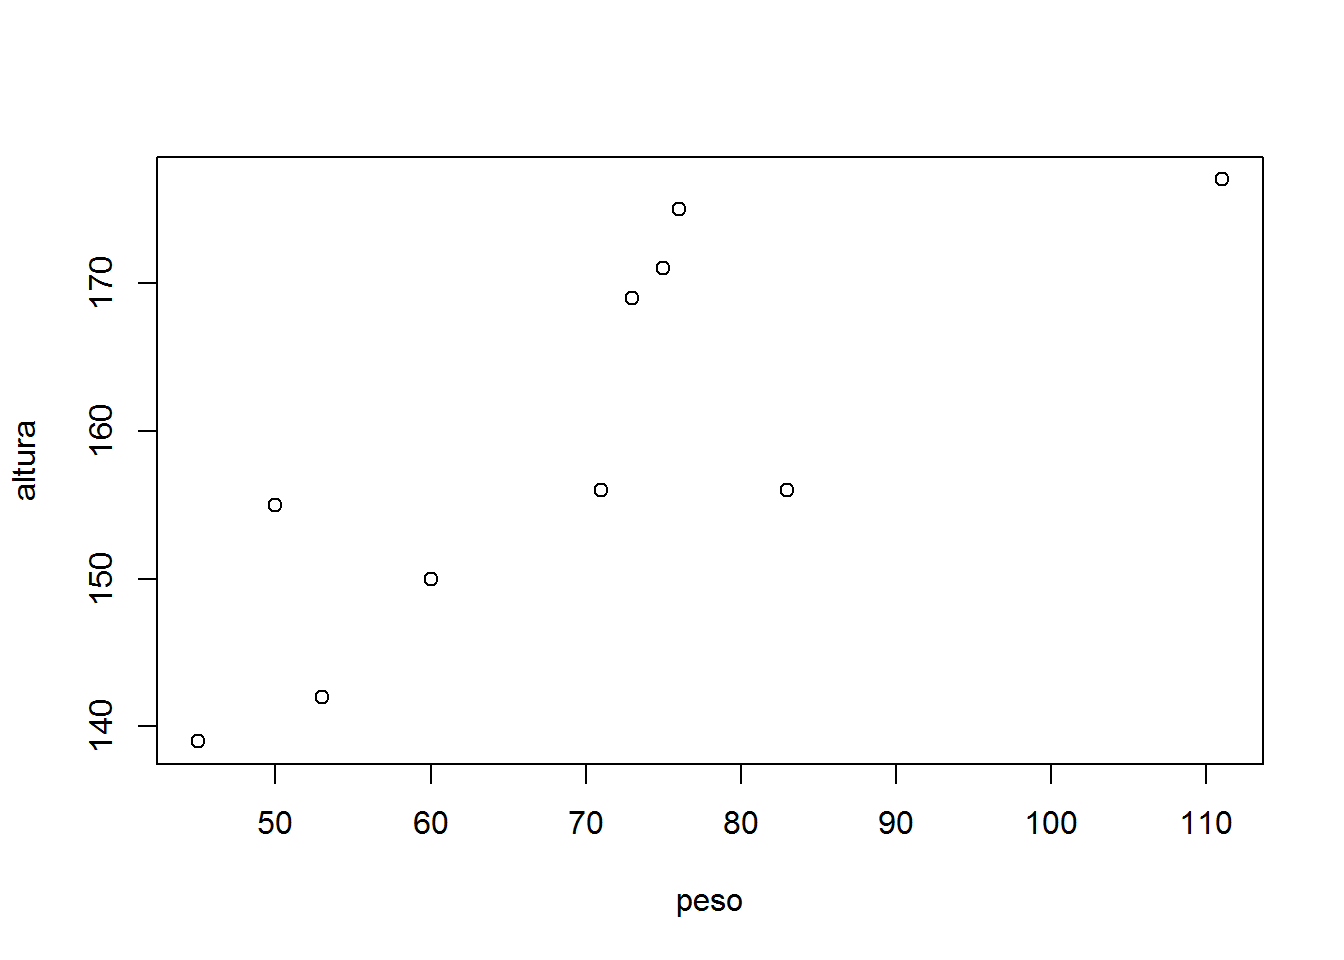
\includegraphics{bookdown-rquer_files/figure-latex/chunk-regli-1.pdf}

\begin{Shaded}
\begin{Highlighting}[]
\KeywordTok{plot}\NormalTok{(peso, altura, }\DataTypeTok{pch =} \DecValTok{16}\NormalTok{, }\DataTypeTok{cex =} \FloatTok{1.3}\NormalTok{, }\DataTypeTok{col =} \StringTok{"orange"}\NormalTok{, }
     \DataTypeTok{main =} \StringTok{"Altura vs Peso"}\NormalTok{, }
     \DataTypeTok{xlab =} \StringTok{"Peso (kg)"}\NormalTok{, }
     \DataTypeTok{ylab =} \StringTok{"Altura (cm)"}\NormalTok{)}
\CommentTok{#modelo lineal}
\KeywordTok{lm}\NormalTok{(altura }\OperatorTok{~}\StringTok{ }\NormalTok{peso) }
\end{Highlighting}
\end{Shaded}

\begin{verbatim}
## 
## Call:
## lm(formula = altura ~ peso)
## 
## Coefficients:
## (Intercept)         peso  
##    120.5135       0.5522
\end{verbatim}

\begin{Shaded}
\begin{Highlighting}[]
\CommentTok{#vemos que el intercept es 120.5135 y el pendiente 0.5522. }
\CommentTok{#Entonces finalmente trazamos la linea que mejor se ajusta (linea de regresión) }
\CommentTok{#en nuestro plot:}
\KeywordTok{abline}\NormalTok{(}\FloatTok{120.5135}\NormalTok{, }\FloatTok{0.5522}\NormalTok{)}
\CommentTok{#o sino también podemos visualizar la linea de regresion con:}
\KeywordTok{abline}\NormalTok{(}\KeywordTok{lm}\NormalTok{(altura }\OperatorTok{~}\StringTok{ }\NormalTok{peso))}
\end{Highlighting}
\end{Shaded}

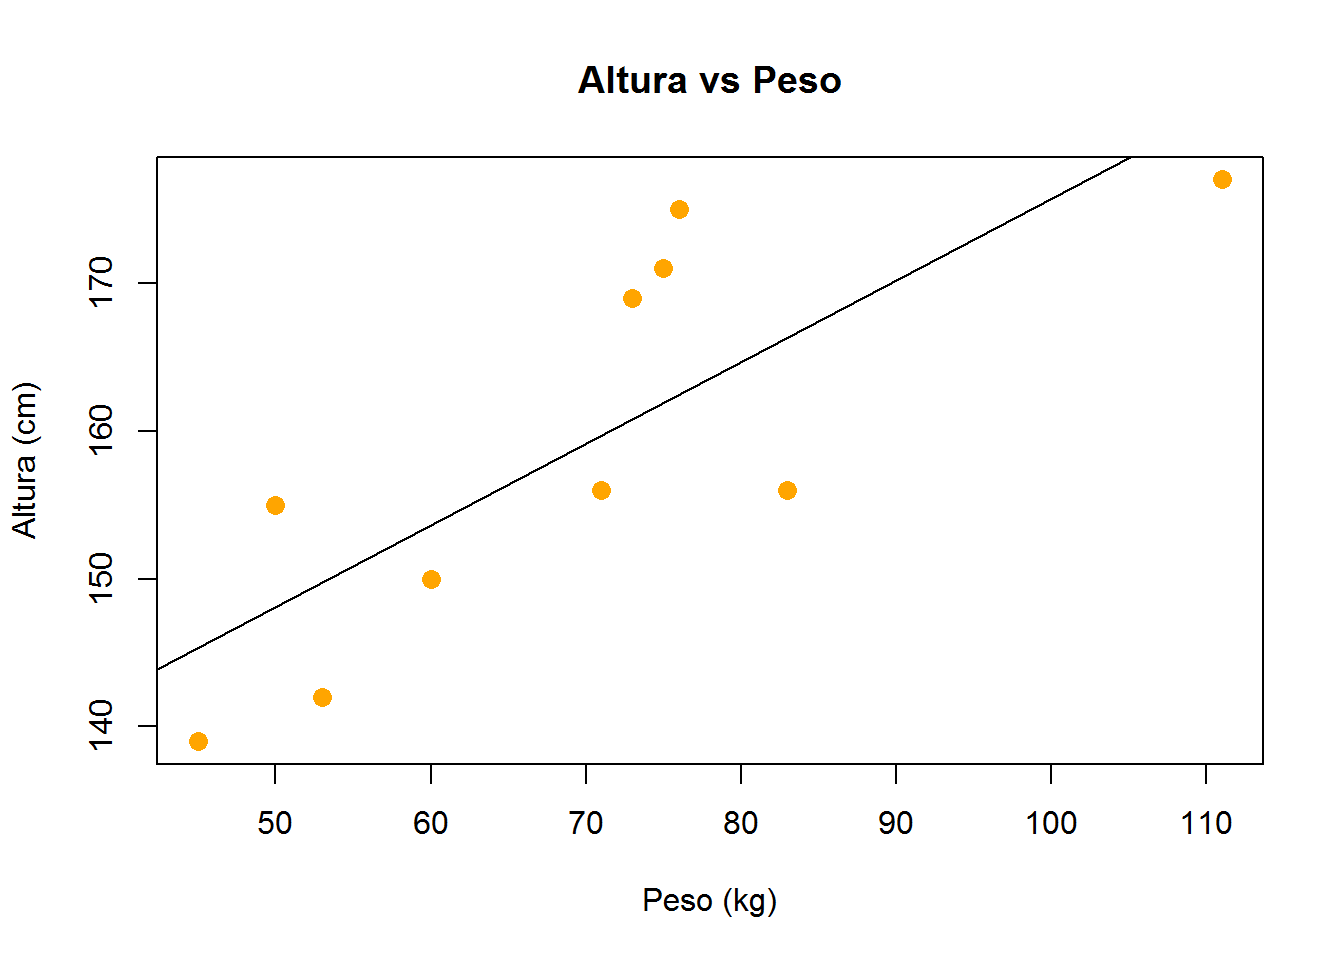
\includegraphics{bookdown-rquer_files/figure-latex/chunk-regli-2.pdf}

\hypertarget{regresion-logistica}{%
\subsection{Regresión logística}\label{regresion-logistica}}

Otro tipo de regresión que nos es útil a menudo es la regresión
logística. Se trata de un modelo de regresión dónde la variable
dependiente es categórica. Por ejemplo: la probabilidad de Aprobar (SI o
NO) un examen en función del número de horas estudiadas, o la
determinación de si un mail es \emph{SPAM} o no en función de varios
atributos o variables independientes (p.ej. el número de palabras, si
contiene imágenes, links, etc.).

El modelo estima, por tanto, la probabilidad de una respuesta binaria
(categórica) en base a uno o más predictores (o variables
independientes) mediante una función logística.

Probemos con un ejemplo tonto en base a nuestros datos: probabilidad de
ser chica en función del número de cromos que tiene una persona.

\begin{Shaded}
\begin{Highlighting}[]
\KeywordTok{library}\NormalTok{(tidyverse)}
\KeywordTok{library}\NormalTok{(ggplot2)}
\NormalTok{misdatos <-}\StringTok{ }\NormalTok{misdatos }\OperatorTok
\CommentTok{#creo la variable Es_Chica}
\StringTok{  }\KeywordTok{mutate}\NormalTok{(}\DataTypeTok{Es_chica =} \KeywordTok{as.numeric}\NormalTok{(Sexo }\OperatorTok{==}\StringTok{ "f"}\NormalTok{))}
\CommentTok{#uso geom_smooth para definir la curva de tendencia de la regresión logística}
\NormalTok{regresion_logistica <-}\StringTok{ }\KeywordTok{ggplot}\NormalTok{(}\DataTypeTok{data =}\NormalTok{ misdatos, }\KeywordTok{aes}\NormalTok{(}\DataTypeTok{x =}\NormalTok{ Cromos,}\DataTypeTok{y =}\NormalTok{ Es_chica)) }\OperatorTok{+}
\StringTok{  }\KeywordTok{geom_smooth}\NormalTok{(}\DataTypeTok{method =} \StringTok{"glm"}\NormalTok{, }\DataTypeTok{method.args =} \KeywordTok{list}\NormalTok{(}\DataTypeTok{family =} \StringTok{"binomial"}\NormalTok{)) }\OperatorTok{+}
\StringTok{  }\KeywordTok{ylab}\NormalTok{(}\StringTok{"¿Es chica? 0(No) -1(Sí)"}\NormalTok{)}
\NormalTok{regresion_logistica}
\end{Highlighting}
\end{Shaded}

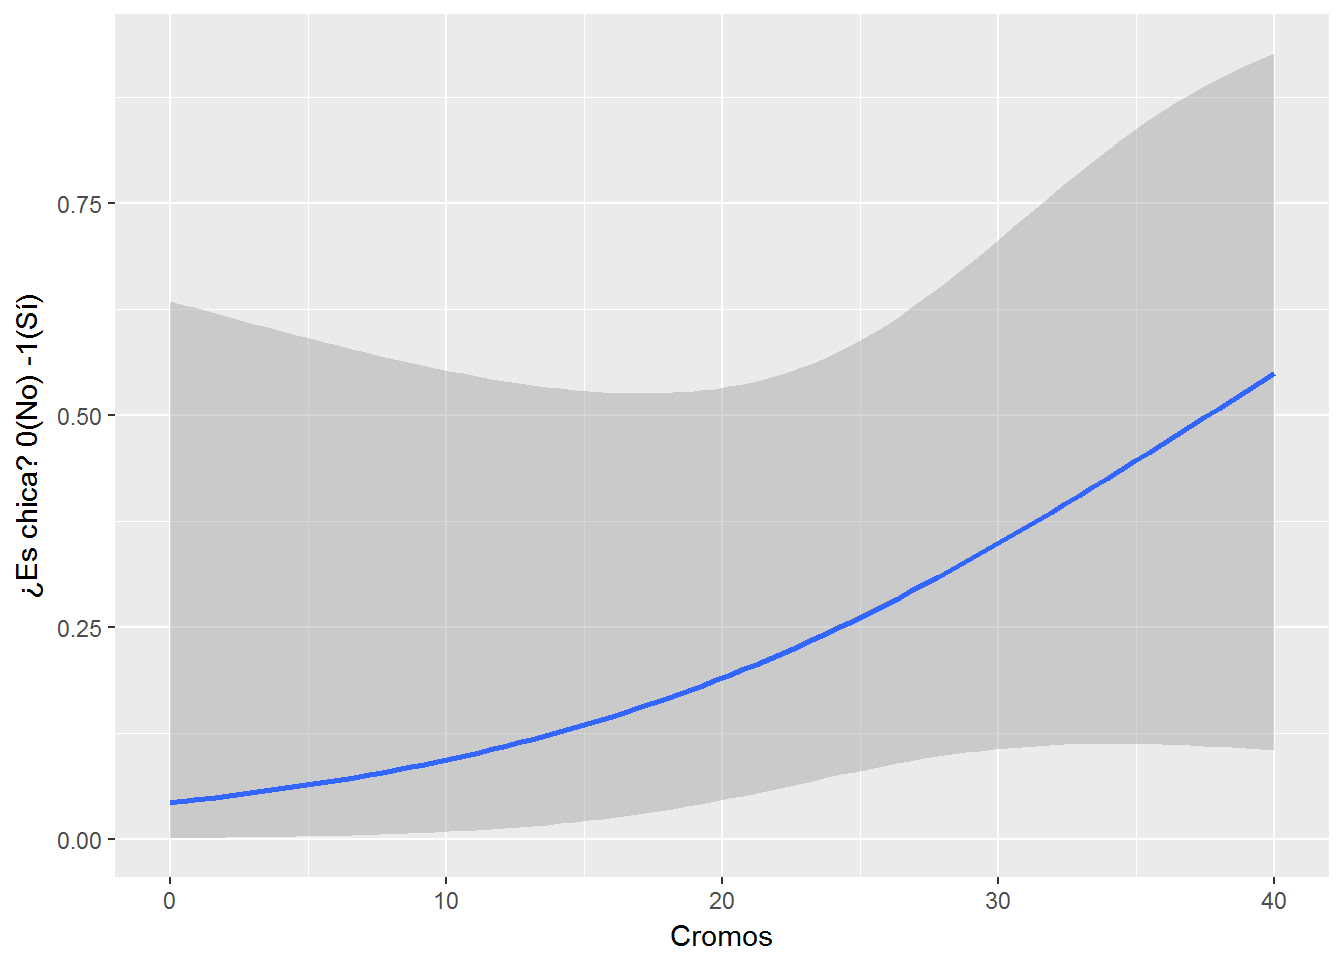
\includegraphics{bookdown-rquer_files/figure-latex/chunk-rlogis-1.pdf}

\hypertarget{proyectar-forecast}{%
\section{Proyectar (Forecast)}\label{proyectar-forecast}}

Veamos ahora otro caso; supongamos que hemos ido anotando desde el año
2000 en un archivo las ventas de cada mes de nuestro negocio. Estaria
bien poder predecir cuáles van a ser las de los proximos meses.

Podemos usar el paquete \textbf{Forecast} \citep{R-forecast}
desarrollado y mantenido por Rob Hyndman, para aplicar modelos
proyectivos conocidos (tales como el modelo ARIMA).

Lo haríamos del siguiente modo:

Leemos los datos a partir de nuestro archivo ventas.csv.

\texttt{df\ \textless{}-\ read.csv("C:/.../ventas.csv")}

Transformamos los datos en un objeto temporal (\emph{time series
object}) del tipo \texttt{ts} (indicamos que los datos son mensuales y
que el periodo de inicio es Enero del 2000).

Mostramos los datos:

\begin{Shaded}
\begin{Highlighting}[]
\NormalTok{df <-}\StringTok{ }\KeywordTok{read.csv}\NormalTok{(}\StringTok{"_bookdown_files/ventas.csv"}\NormalTok{)}
\NormalTok{series <-}\StringTok{ }\KeywordTok{ts}\NormalTok{(df, }\DataTypeTok{frequency =} \DecValTok{12}\NormalTok{, }\DataTypeTok{start =} \KeywordTok{c}\NormalTok{(}\DecValTok{2000}\NormalTok{,}\DecValTok{1}\NormalTok{))}
\KeywordTok{print}\NormalTok{(series)}
\end{Highlighting}
\end{Shaded}

\begin{verbatim}
##        Jan   Feb   Mar   Apr   May   Jun   Jul   Aug   Sep   Oct   Nov
## 2000  6938  7524  8475  9401  9558  9182  9103 10513  9573 10254 11187
## 2001  7502  7524  8766  9867 10063  9635  9794 10628 10013 10346 11760
## 2002  7280  7902  9921  9869 10009  9893  9735 11157 10217 10730 12354
## 2003  7518  7961  9815 10168 10620 10301  9784 11264 10710 10439 12751
## 2004  7684  8991 10349 10570 11405 10554 10202 12134 10623 11250 12875
## 2005  8194  8835 10840 10131 11505 10654 10734 12461 10942 11635 13244
## 2006  8800  9499 10863 11825 12239 11451 11633 12971 11214 12384 13854
## 2007  9237 10171 12081 12386 13167 12280 12461 13734 12357 12948 14643
## 2008  9447 11170 12841 13124 13735 12953 12500 14610 13375 13369 15675
## 2009 10060 11450 13067 13362 13787 12935 12600 14818 12104 13218 15352
## 2010 10344 11730 13977 13195 14150 13210 12873 15113 12445 14006 15911
## 2011 10804 11662 13452 13691 14730 13496 13854 15522 13567 14601 16555
## 2012 11790 13344 14760 15058 15379 14237 14667 15588 14224 15570 17230
## 2013 12046 13878 15727 15708 15989 15559 15218 16697 14960 16509 18402
## 2014 12893 14474 16386 16848 17103 16505 16275 17832 16767 17253 19391
## 2015 13927 15077 18045 17096 18474 17289 16883 18850 16765 17614 20550
## 2016 14170 15877 17764 17098 19081 17006 17366 19038 15881 16791 18753
## 2017 13382 14681 15560 16334 17260 15429 16002 17650 15624 17046 18324
##        Dec
## 2000 18395
## 2001 18851
## 2002 20016
## 2003 20002
## 2004 19944
## 2005 21118
## 2006 22418
## 2007 24286
## 2008 24875
## 2009 24534
## 2010 25350
## 2011 26760
## 2012 28406
## 2013 30276
## 2014 31462
## 2015 30635
## 2016 26718
## 2017 27110
\end{verbatim}

Ploteamos la serie temporal. Nos aseguramos que el eje \texttt{y}
empieza por cero.

\begin{Shaded}
\begin{Highlighting}[]
\KeywordTok{plot}\NormalTok{(series, }\DataTypeTok{ylim =} \KeywordTok{c}\NormalTok{(}\DecValTok{0}\NormalTok{, }\DecValTok{35000}\NormalTok{))}
\end{Highlighting}
\end{Shaded}

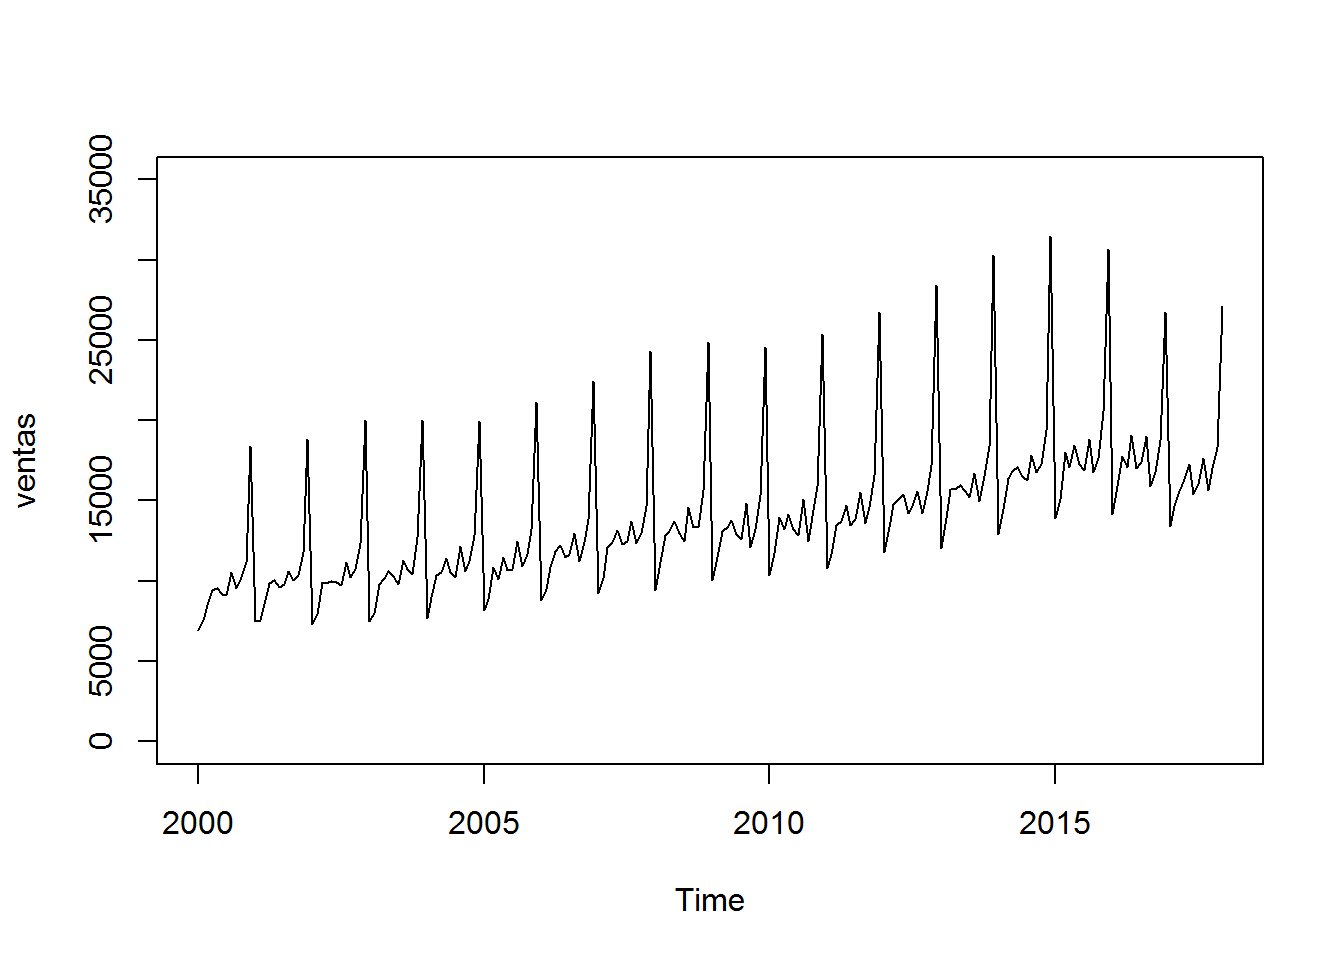
\includegraphics{bookdown-rquer_files/figure-latex/chunk-plotseries-1.pdf}

Generemos ahora una prevision para los próximos 20 periodos en base al
modelo ARIMA. Lo hacemos en dos pasos: 1) creamos un modelo usando la
función \texttt{auto.arima} del paquete \texttt{forecast} 2) generamos
una proyección en base al modelo usando la función \texttt{forecast}

Representamos gráficamente la previsión:

\begin{Shaded}
\begin{Highlighting}[]
\KeywordTok{require}\NormalTok{(forecast)}
\NormalTok{model_arima <-}\StringTok{ }\KeywordTok{auto.arima}\NormalTok{(series)}
\NormalTok{fcast_arima <-}\StringTok{ }\KeywordTok{forecast}\NormalTok{(model_arima, }\DataTypeTok{h =} \DecValTok{20}\NormalTok{)}
\KeywordTok{plot}\NormalTok{(fcast_arima)}
\end{Highlighting}
\end{Shaded}

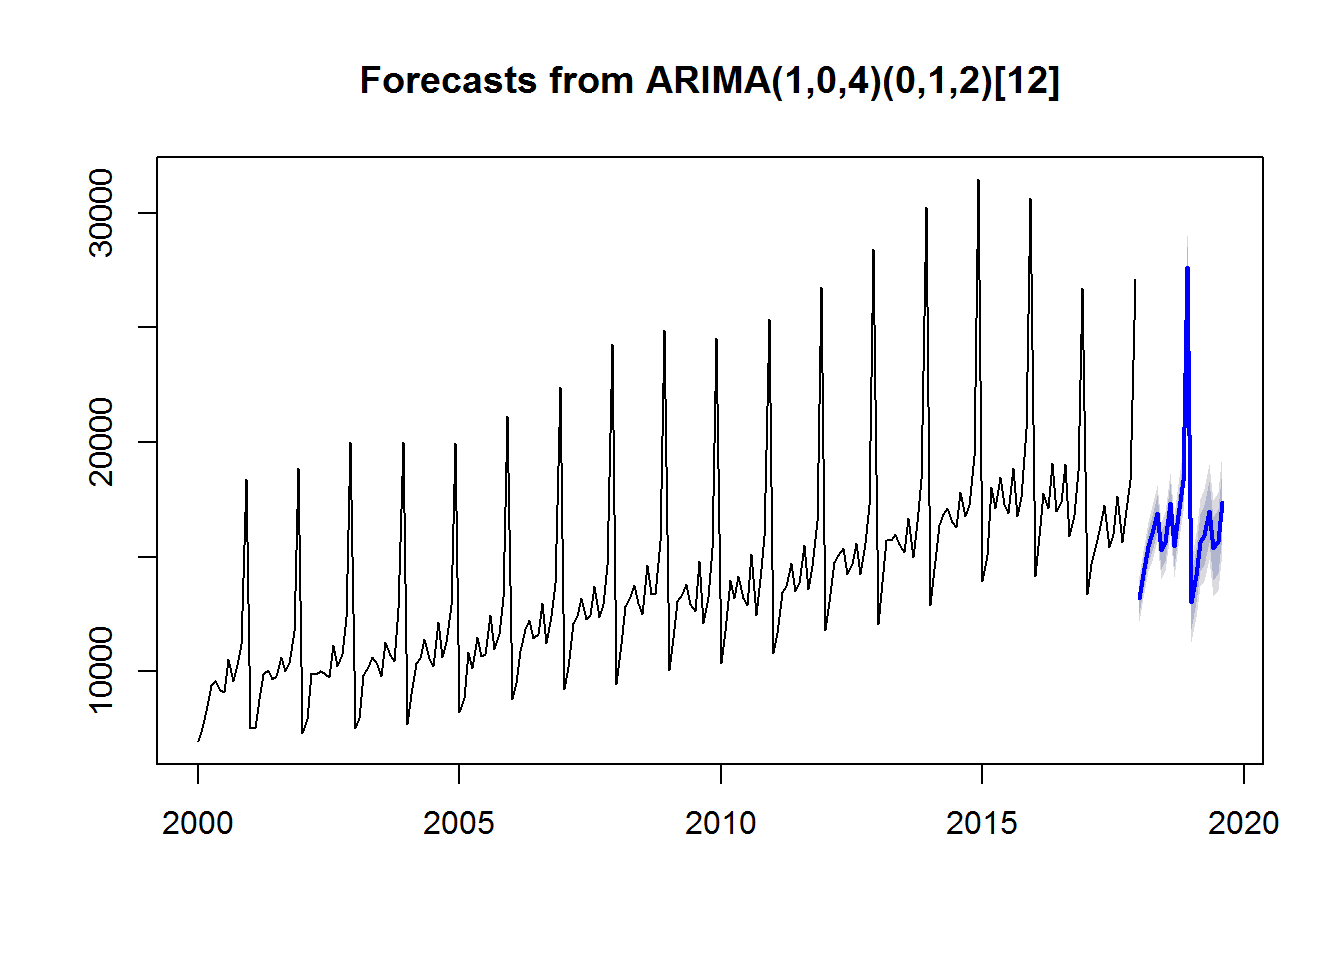
\includegraphics{bookdown-rquer_files/figure-latex/chunk-forecast-1.pdf}

\hypertarget{r-para-visualizar}{%
\chapter{R para Visualizar}\label{r-para-visualizar}}

\begin{quote}
``There is no such thing as information overload. There is only bad
design\ldots{}.''

--- Edward Tufte
\end{quote}

En este capítulo veremos algunas opciones básicas para visualizar
convenientemente nuestros datos.

\hypertarget{graficos-de-dispersion}{%
\section{Gráficos de dispersión}\label{graficos-de-dispersion}}

Una primera forma de visualización, útil en muchos casos son los
\textbf{gráficos de dispersión} o \emph{scatterplots} en inglés. Para
generar muchos tipos de visualizaciones nos será sumamente útil el
paquete \textbf{ggplot2} \citep{R-ggplot2} creado por el señor
\href{http://hadley.nz/}{Hadley Wickham}. Lo primero, cargémoslo:

\begin{Shaded}
\begin{Highlighting}[]
\KeywordTok{library}\NormalTok{(ggplot2) }
\end{Highlighting}
\end{Shaded}

La opción más sencilla para visualizar nuestros datos es usar la función
\texttt{qplot} dónde en los argumentos de la función pongo: la variable
que quiero en el eje X, la que quiero en el eje Y, seguido de la tabla
de los datos que estoy analizando (misdatos):

\begin{Shaded}
\begin{Highlighting}[]
\KeywordTok{qplot}\NormalTok{(Cromos, Edad, }\DataTypeTok{data =}\NormalTok{ misdatos)}
\end{Highlighting}
\end{Shaded}

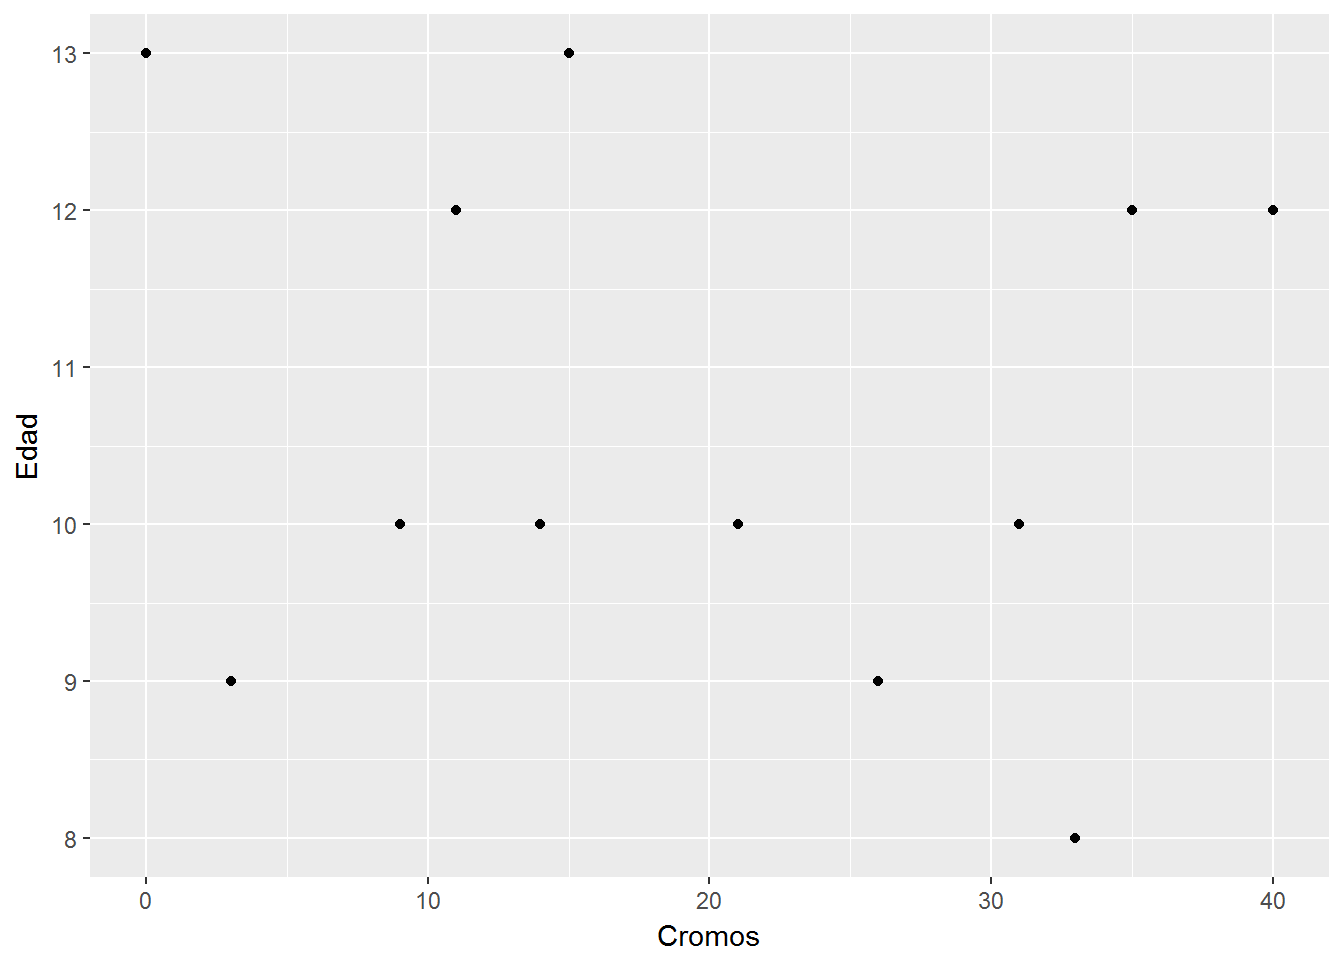
\includegraphics{bookdown-rquer_files/figure-latex/chunk-simpleqplot-1.pdf}

Puedo añadir una tercera variable (Nombre) para representarla por
ejemplo mediante color:

\begin{Shaded}
\begin{Highlighting}[]
\KeywordTok{qplot}\NormalTok{(Cromos, Edad, }\DataTypeTok{data =}\NormalTok{ misdatos, }\DataTypeTok{color =}\NormalTok{ Nombre)}
\end{Highlighting}
\end{Shaded}

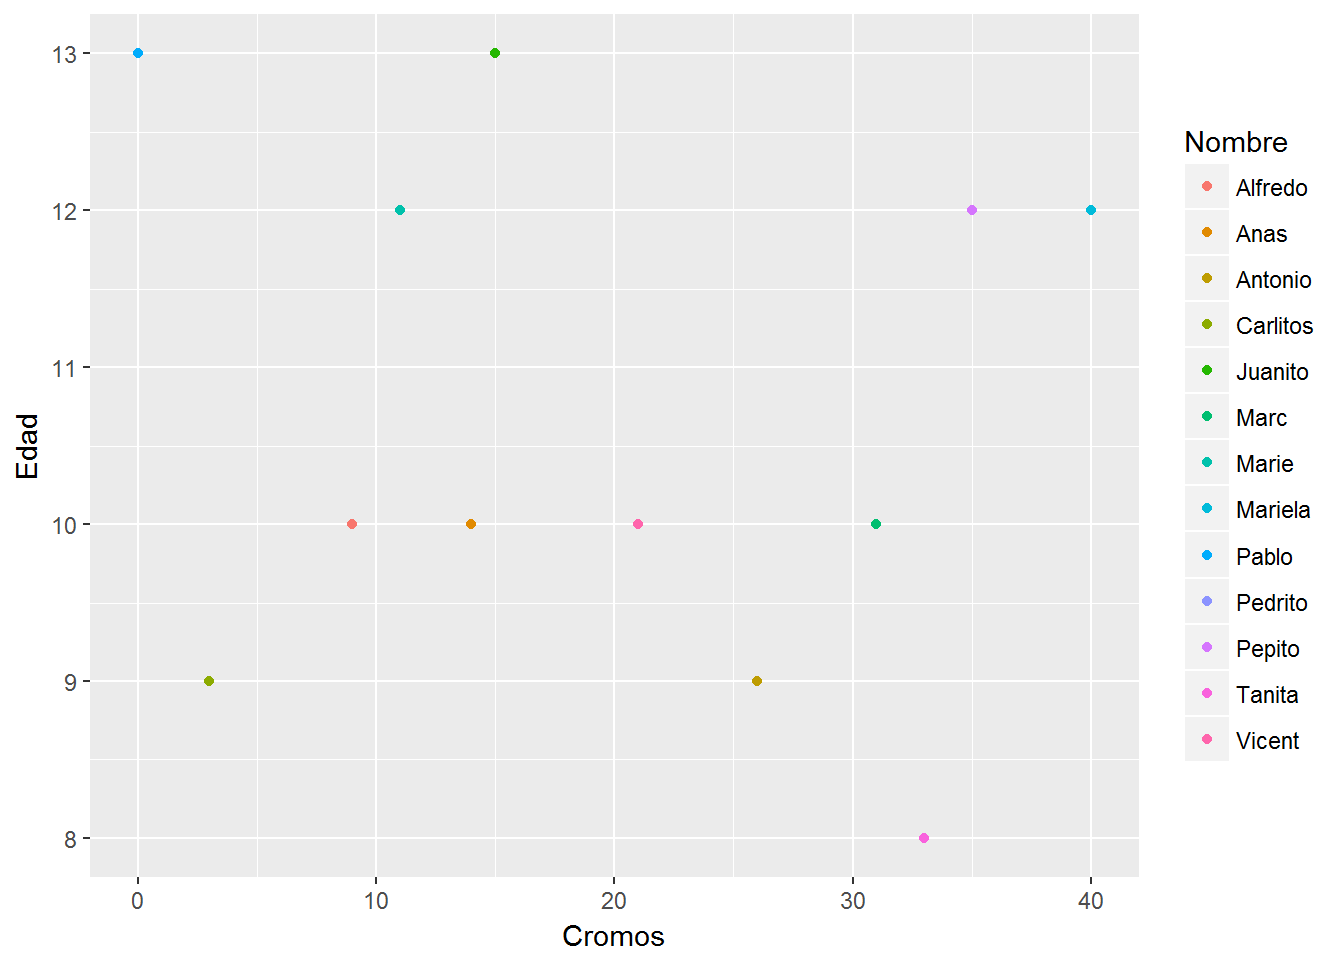
\includegraphics{bookdown-rquer_files/figure-latex/chunk-qplotcolor-1.pdf}

(nótese que la leyenda se me crea automáticamente).

Otra utilidad conveniente a menudo a la hora de visualizar nuestros
datos es hacer varias capas o particiones ( \textbf{facets} ) para
mostrar los datos en función de determinadas variables. Veámoslos por
ejemplo en función del deporte practicado.

\begin{Shaded}
\begin{Highlighting}[]
\KeywordTok{qplot}\NormalTok{(Cromos, Edad, }\DataTypeTok{data =}\NormalTok{ misdatos, }\DataTypeTok{color =}\NormalTok{ Nombre, }\DataTypeTok{facets =}\NormalTok{ .}\OperatorTok{~}\NormalTok{Deporte)}
\end{Highlighting}
\end{Shaded}

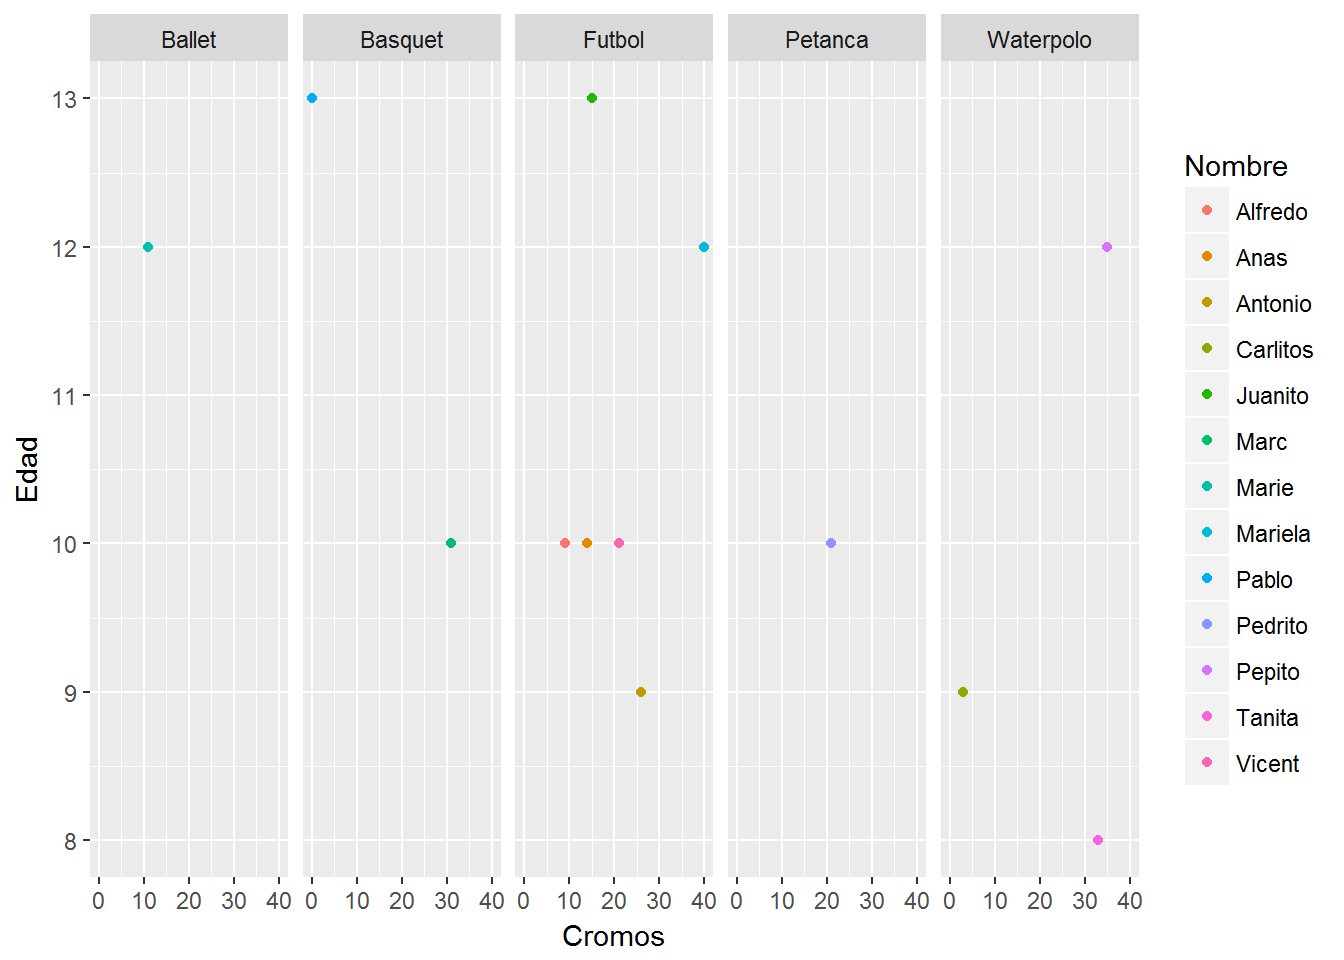
\includegraphics{bookdown-rquer_files/figure-latex/chunk-qplotfacet1-1.pdf}

La opción \texttt{qplot} está bien para generar visualizaciones rápidas
de nuestros datos, pero cuando queremos tener más control estético
podemos usar la expresión \texttt{ggplot} seguida de los datos y a
continuación los parámetros estéticos que deseemos (que indicamos con
\texttt{aes()}), más la forma (\texttt{geom}) de los datos (sean puntos,
barras u otras formas).

\begin{Shaded}
\begin{Highlighting}[]
\NormalTok{plot <-}\StringTok{ }\KeywordTok{ggplot}\NormalTok{(misdatos, }\KeywordTok{aes}\NormalTok{ (Cromos, Edad)) }\OperatorTok{+}\StringTok{ }\KeywordTok{geom_point}\NormalTok{()}
\NormalTok{plot}
\end{Highlighting}
\end{Shaded}

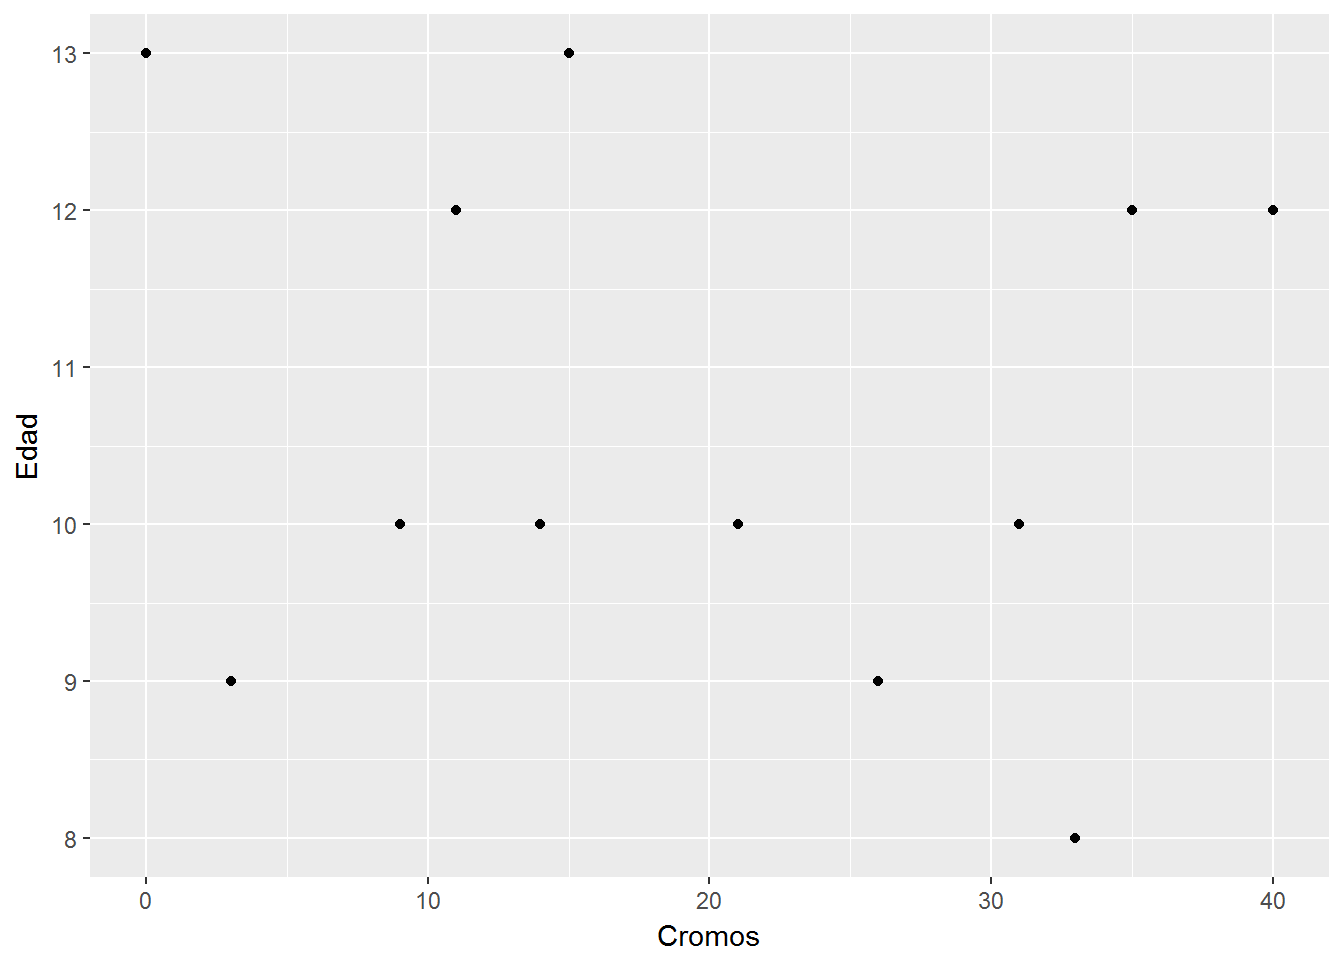
\includegraphics{bookdown-rquer_files/figure-latex/chunk-ggplotgeom-1.pdf}

Así, por ejemplo puedo añadir estética de color a los puntos, bien como
una constante:

\begin{Shaded}
\begin{Highlighting}[]
\NormalTok{plot <-}\StringTok{ }\KeywordTok{ggplot}\NormalTok{(misdatos, }\KeywordTok{aes}\NormalTok{ (Cromos, Edad)) }\OperatorTok{+}\StringTok{ }\KeywordTok{geom_point}\NormalTok{(}\DataTypeTok{color =} \StringTok{"steelblue"}\NormalTok{)}
\NormalTok{plot}
\end{Highlighting}
\end{Shaded}

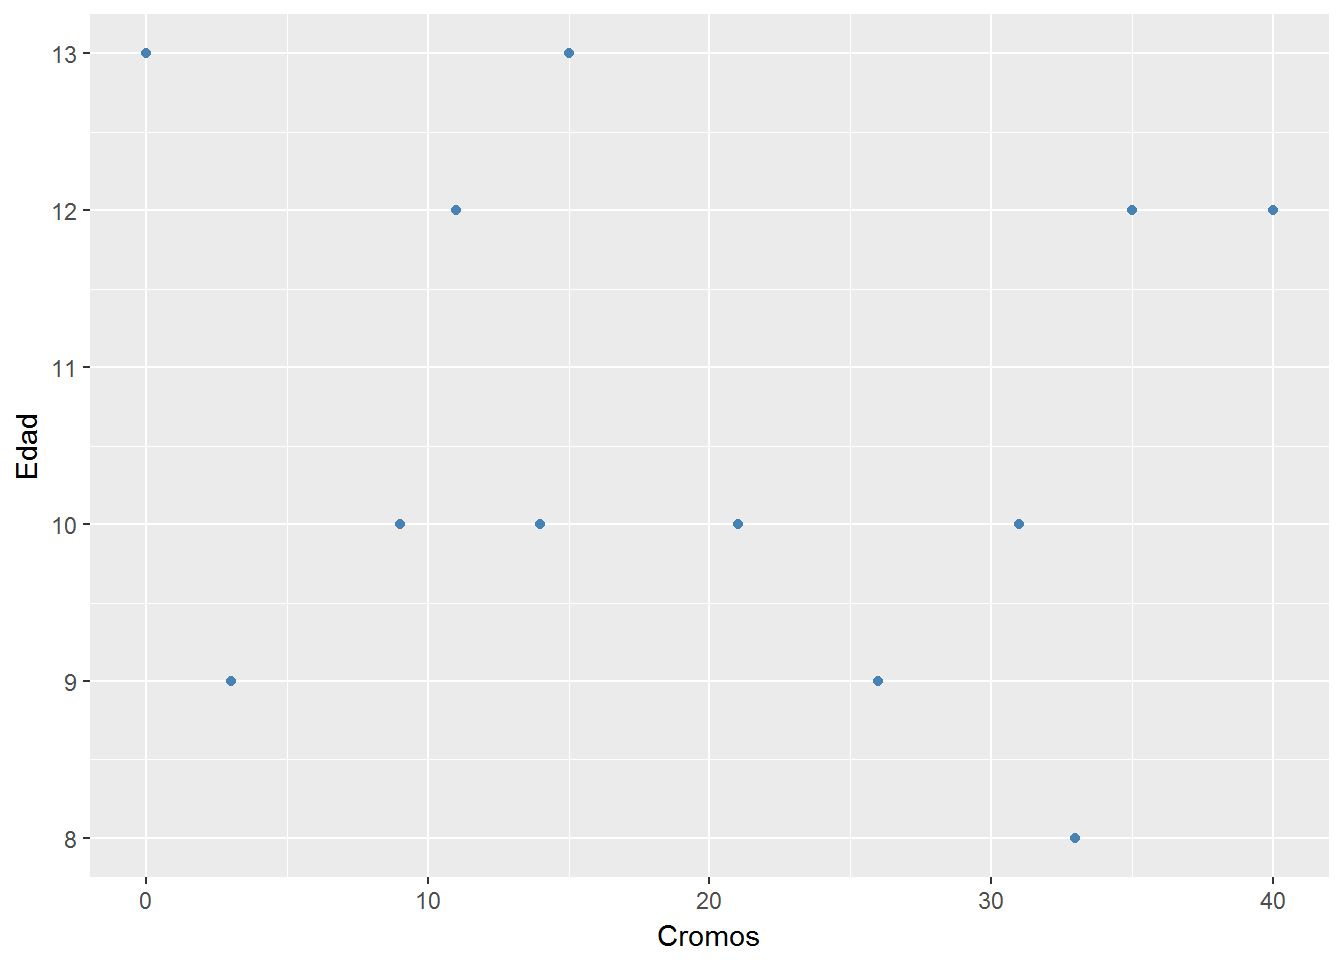
\includegraphics{bookdown-rquer_files/figure-latex/chunk-geomconstant-1.pdf}

o bien como una variable (dónde el color es función del Sexo):

\begin{Shaded}
\begin{Highlighting}[]
\NormalTok{plot <-}\StringTok{ }\KeywordTok{ggplot}\NormalTok{(misdatos, }\KeywordTok{aes}\NormalTok{ (Cromos, Edad)) }\OperatorTok{+}\StringTok{ }\KeywordTok{geom_point}\NormalTok{(}\KeywordTok{aes}\NormalTok{(}\DataTypeTok{color =}\NormalTok{ Sexo))}
\NormalTok{plot}
\end{Highlighting}
\end{Shaded}

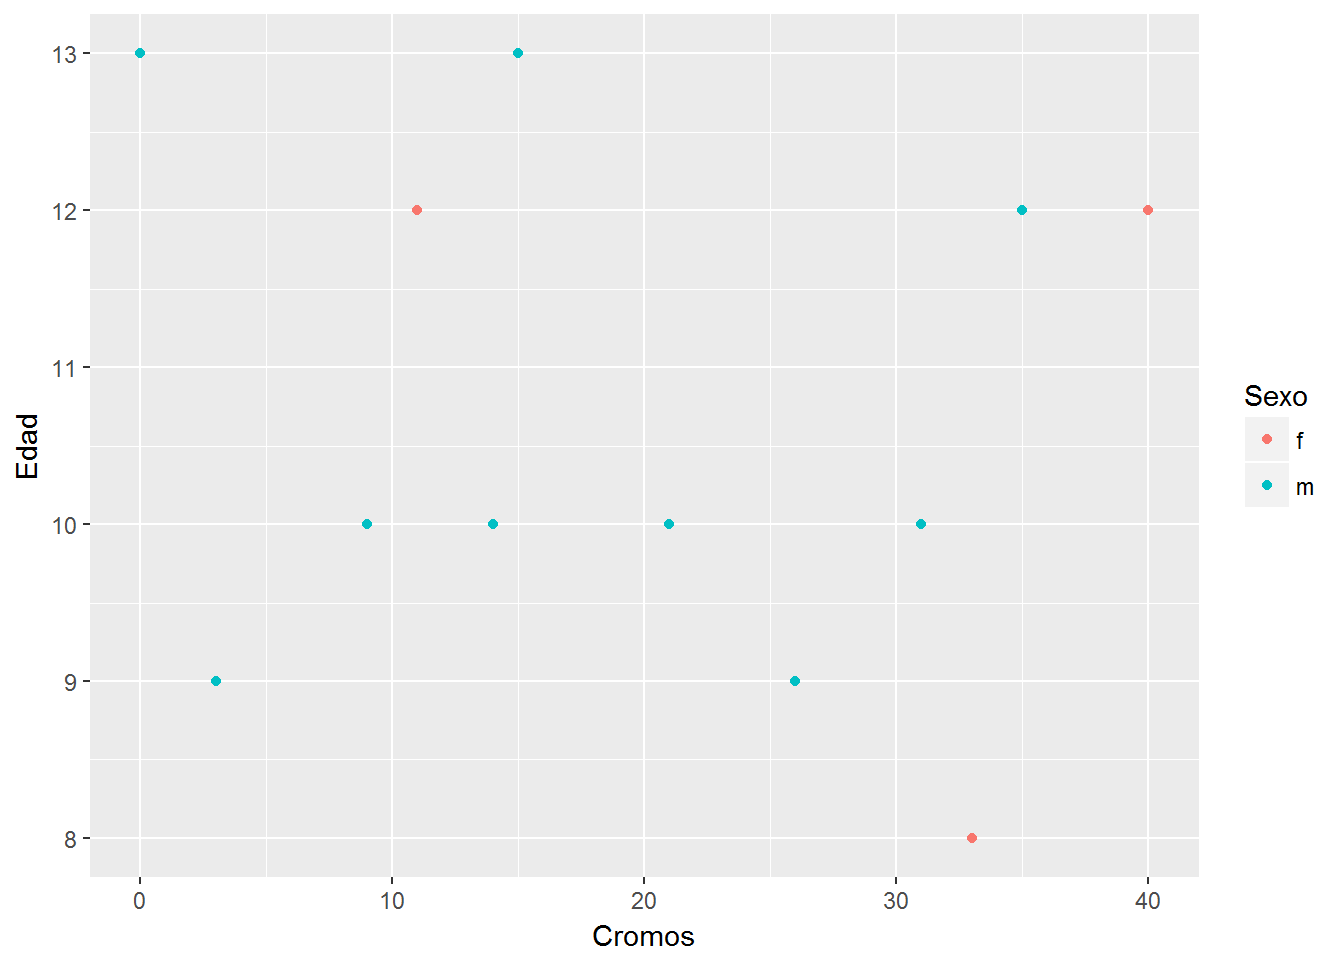
\includegraphics{bookdown-rquer_files/figure-latex/chunk-geomvariable-1.pdf}

O el tamaño (size) es función del número de hermanos:

\begin{Shaded}
\begin{Highlighting}[]
\NormalTok{plot <-}\StringTok{ }\KeywordTok{ggplot}\NormalTok{(misdatos, }\KeywordTok{aes}\NormalTok{ (Cromos, Edad)) }\OperatorTok{+}\StringTok{ }\KeywordTok{geom_point}\NormalTok{(}\KeywordTok{aes}\NormalTok{(}\DataTypeTok{size =}\NormalTok{ numerodehermanos))}
\NormalTok{plot}
\end{Highlighting}
\end{Shaded}

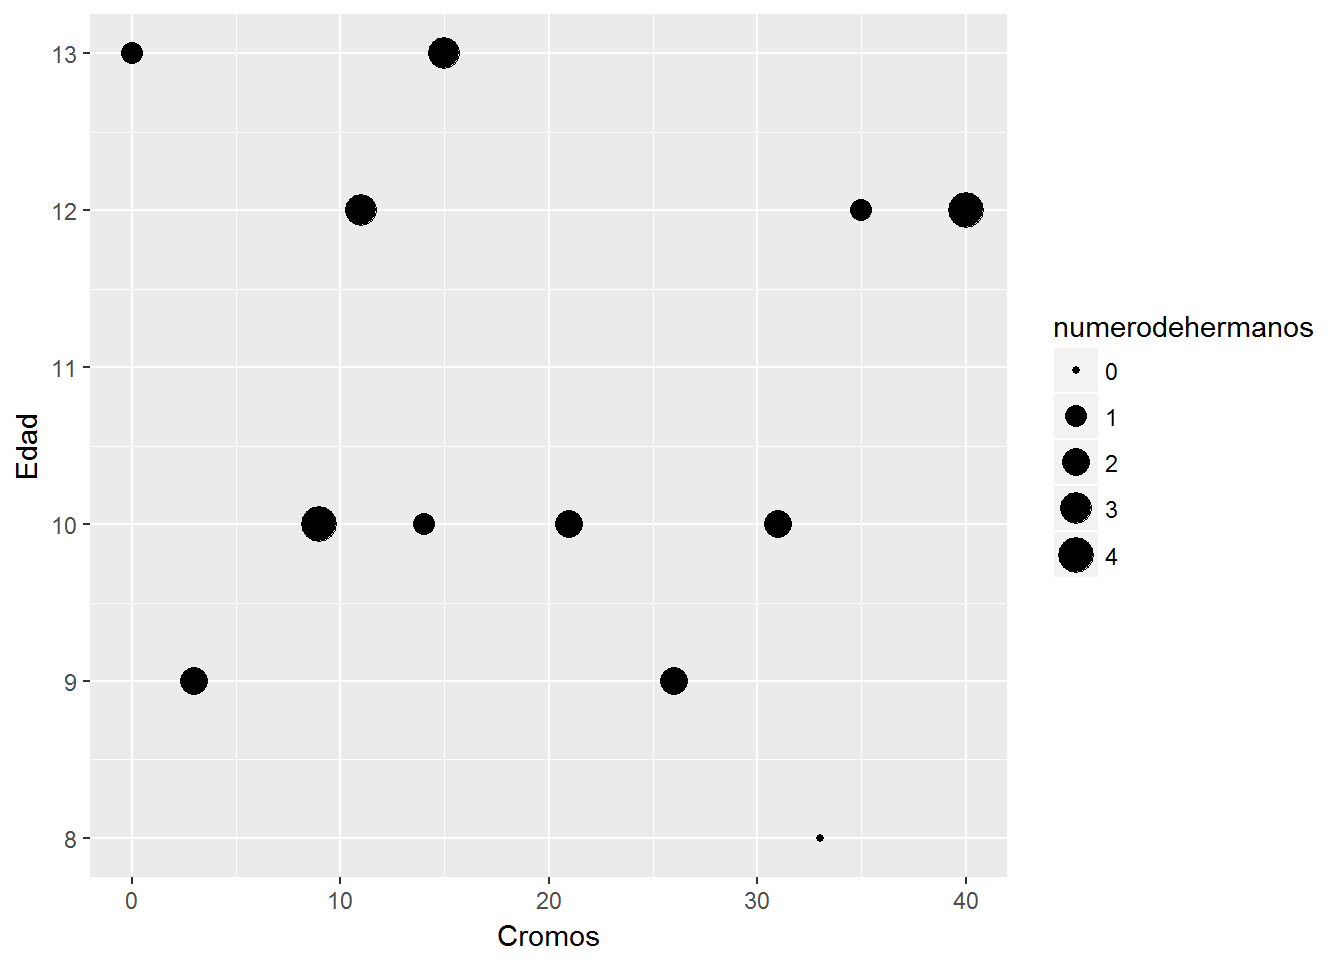
\includegraphics{bookdown-rquer_files/figure-latex/chunk-geomvariablesize-1.pdf}

O ambos color y tamaño son función del sexo y del número de hermanos
respectivamente y además la forma es función del Deporte practicado:

\begin{Shaded}
\begin{Highlighting}[]
\NormalTok{plot <-}\StringTok{ }\KeywordTok{ggplot}\NormalTok{(misdatos, }\KeywordTok{aes}\NormalTok{ (Cromos, Edad)) }\OperatorTok{+}\StringTok{ }\KeywordTok{geom_point}\NormalTok{(}\KeywordTok{aes}\NormalTok{(}\DataTypeTok{color =}\NormalTok{ Sexo, }\DataTypeTok{size =}\NormalTok{ numerodehermanos, }\DataTypeTok{shape =}\NormalTok{ Deporte))}
\NormalTok{plot}
\end{Highlighting}
\end{Shaded}

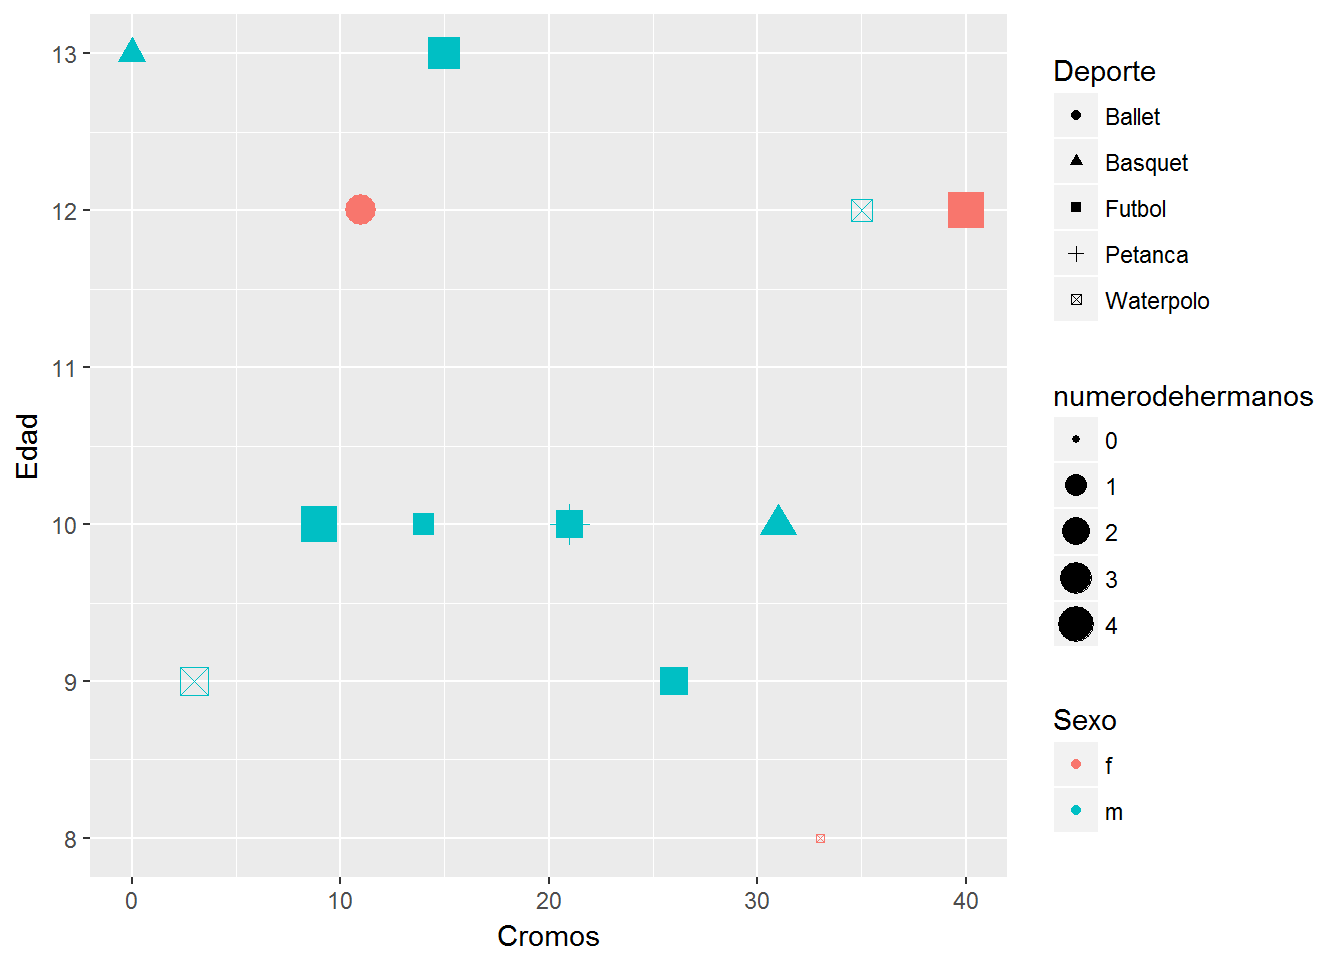
\includegraphics{bookdown-rquer_files/figure-latex/chunk-geomvariablesizecolor-1.pdf}

\hypertarget{histogramas}{%
\section{Histogramas}\label{histogramas}}

Para representar un histograma simplemente usariamos en este caso en
nuestra expresión la forma estética \texttt{geom\_histogram}.

\begin{Shaded}
\begin{Highlighting}[]
\KeywordTok{library}\NormalTok{(ggplot2)}
\KeywordTok{ggplot}\NormalTok{(misdatos, }\KeywordTok{aes}\NormalTok{(numerodehermanos)) }\OperatorTok{+}
\StringTok{  }\KeywordTok{geom_histogram}\NormalTok{(}\DataTypeTok{binwidth =} \FloatTok{.5}\NormalTok{, }\DataTypeTok{fill =} \StringTok{"Steelblue"}\NormalTok{, }\DataTypeTok{show.legend =} \OtherTok{FALSE}\NormalTok{)}
\end{Highlighting}
\end{Shaded}

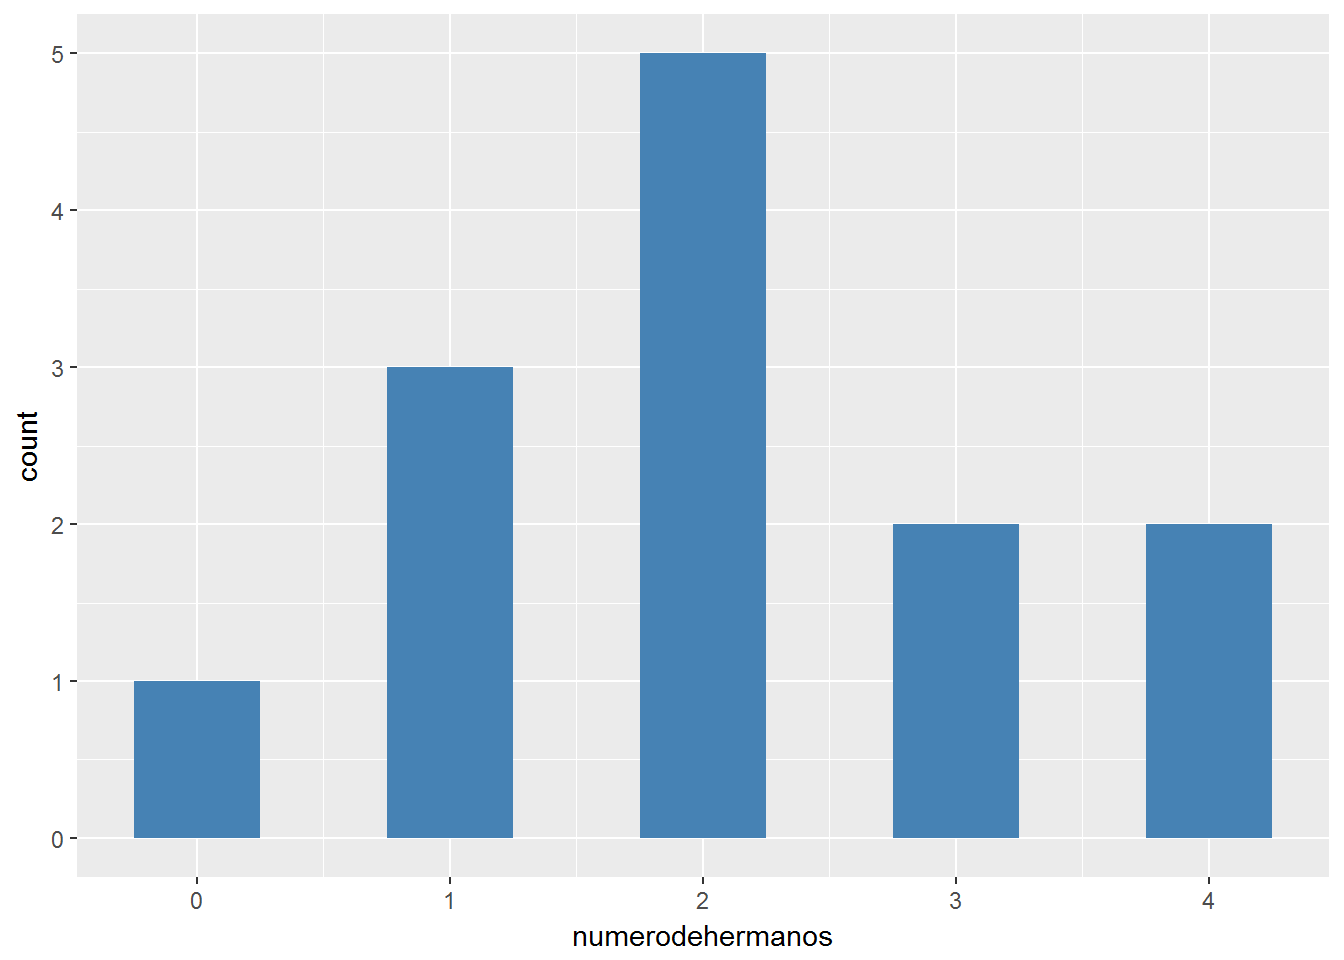
\includegraphics{bookdown-rquer_files/figure-latex/chunk-histogram-1.pdf}

Nótese que a efectos estéticos hemos representado el histograma
ajustando el ancho de las barras (con \texttt{binwidth}) y rellendando
de color (con \texttt{fill}).

\hypertarget{redes}{%
\section{Redes}\label{redes}}

Eventualmente puede ser interesante visualizar datos que describen una
red y percibir su estructura relacional.

Con el paquete \textbf{igraph} \citep{R-igraph} podemos leer una red
cuya información tengamos expresada en forma de nodos y enlaces.

En nuestro caso partimos de un arxivo de nodos que es una tabla de
nombres de personas y un archivo de enlaces que es una tabla con tres
columnas (nombre de una persona, nombre de otra persona con quien
interacciona y número de cromos intercambiados).

\begin{Shaded}
\begin{Highlighting}[]
\CommentTok{#cargamos el paquete igraph}
\KeywordTok{library}\NormalTok{(igraph)}

\CommentTok{#leemos archivos de nodos y de enlaces que tenemos en nuestro directorio}
\NormalTok{nodos <-}\StringTok{ }\KeywordTok{read.csv}\NormalTok{(}\StringTok{"_bookdown_files/grafo_nodos.csv"}\NormalTok{, }\DataTypeTok{header =}\NormalTok{ T, }\DataTypeTok{as.is =}\NormalTok{ T)}
\NormalTok{enlaces <-}\StringTok{ }\KeywordTok{read.csv}\NormalTok{(}\StringTok{"_bookdown_files/grafo_enlaces.csv"}\NormalTok{, }\DataTypeTok{header =}\NormalTok{ T, }\DataTypeTok{as.is =}\NormalTok{ T)}
\end{Highlighting}
\end{Shaded}

Ahora podemos visualizar la red con el paquete \texttt{igraph}.

\begin{Shaded}
\begin{Highlighting}[]
\CommentTok{#trasformamos los datos en objetos de red mediante la función graph.data.frame}
\NormalTok{red <-}\StringTok{ }\KeywordTok{graph.data.frame}\NormalTok{(enlaces, }\DataTypeTok{directed =} \OtherTok{TRUE}\NormalTok{, }\DataTypeTok{vertices =}\NormalTok{ nodos)}

\CommentTok{#representamos el grafo especificando varios criterios estéticos}

\KeywordTok{plot}\NormalTok{(red, }\DataTypeTok{layout =}\NormalTok{ layout.fruchterman.reingold, }\DataTypeTok{vertex.size =} \DecValTok{9}\NormalTok{, }
     \DataTypeTok{vertex.label.color =} \StringTok{"grey20"}\NormalTok{, }\DataTypeTok{vertex.label.dist =} \FloatTok{0.9}\NormalTok{, }
     \DataTypeTok{vertex.color =} \StringTok{"Steelblue"}\NormalTok{, }\DataTypeTok{vertex.frame.color =} \StringTok{"white"}\NormalTok{, }
     \DataTypeTok{edge.arrow.size =} \FloatTok{0.5}\NormalTok{, }\DataTypeTok{edge.curved =} \DecValTok{0}\NormalTok{, }\DataTypeTok{vertex.label.font =} \DecValTok{9}\NormalTok{, }
     \DataTypeTok{vertex.label.cex =} \FloatTok{0.8}\NormalTok{)}
\end{Highlighting}
\end{Shaded}

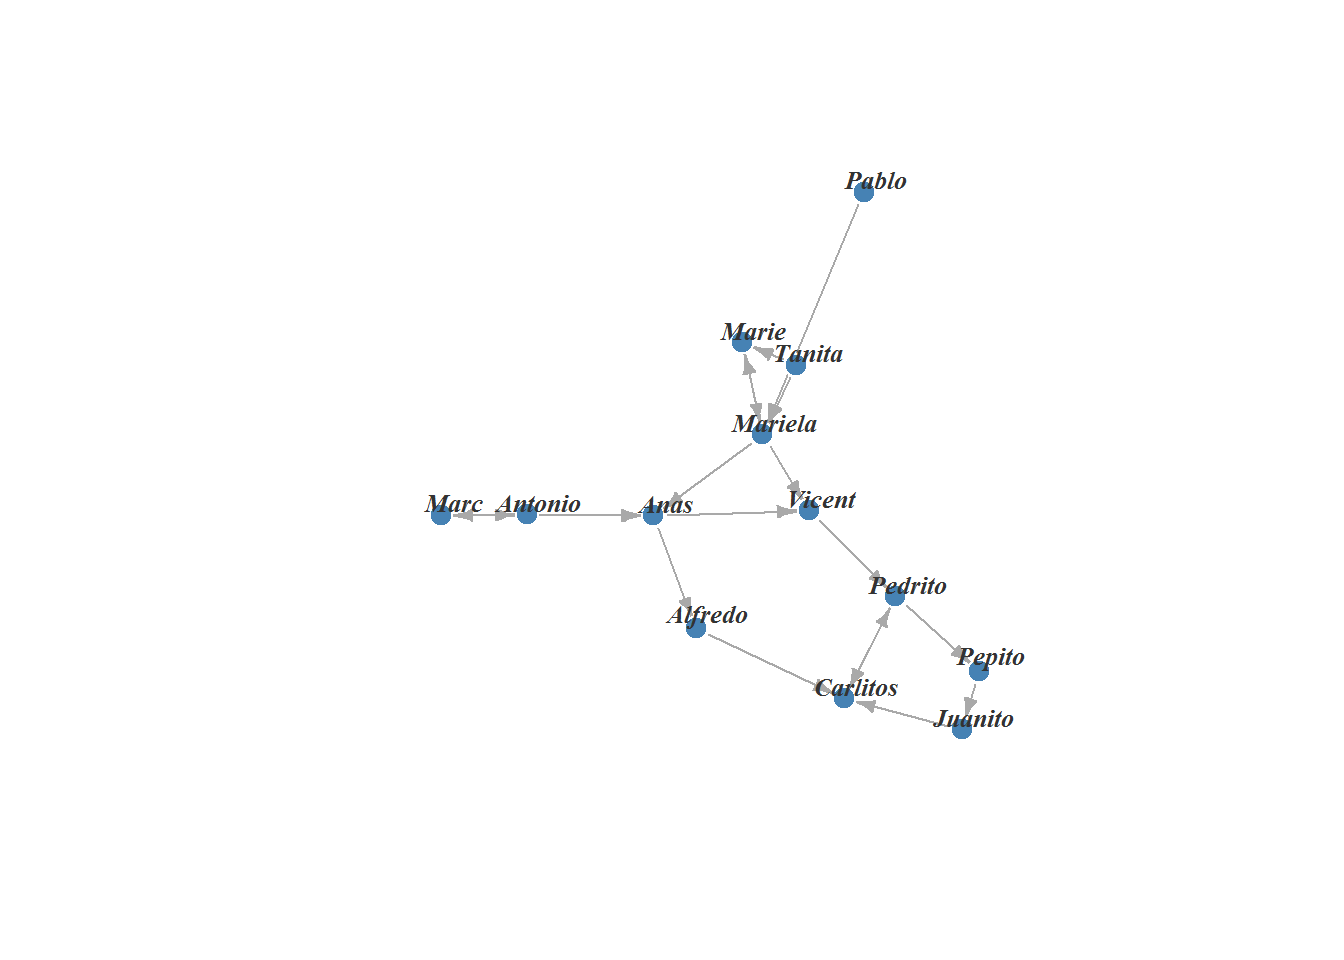
\includegraphics{bookdown-rquer_files/figure-latex/chunk-plotnetwork-1.pdf}

Apreciamos un grafo resultante cuyos nodos son los nombres de las
personas y los enlaces los vínculos que éstas establecen (en este caso
intercambio de cromos).

Podemos llegar a hacer grafos mucho más sofisticados que este: reflejar
varias variables en ellos, distintos layouts, aplicar conceptos de la
teoría de grafos (centralidad, cercanía, intermediacion) para
entenderlos mejor, etc.

Nota: para aprender más acerca de representaciones de redes con R
recomiendo leer los excelentes materiales al respecto de
\href{https://kateto.net/}{Katya Ognyanova}; más recientemente
\href{https://www.data-imaginist.com/}{Tomas Lin Pedersen} ha aumentado
considerablemente las posibilidades de trabajar con grafos en R, con la
creación de los paquetes integrados de manipulación y visualización de
grafos \textbf{ggraph} \citep{R-ggraph} y \textbf{tidygraph}
\citep{R-tidygraph}. Si te interesan los grafos te aconsejo estar al
tanto de su evolución.

\hypertarget{mapas-geograficos}{%
\section{Mapas geográficos}\label{mapas-geograficos}}

También podemos representar en R mapas geográficos de varios modos;
usamos paquetes como \textbf{ggmap} \citep{R-ggmap}, \textbf{tmap}
\citep{R-tmap} para representar los mapas y luego con paquetes como por
ejemplo \textbf{rgdal} \citep{R-rgdal} podemos importar perímetros
geoespaciales de áreas geográficas o países (en forma de
\emph{shapefiles}) en R y localizarlos en el mapa con nuestros datos.

Por ejemplo, podemos generar rápidamente un mapa de Europa con
\texttt{tmap} con sólo indicar una región geográfica:

\begin{Shaded}
\begin{Highlighting}[]
\KeywordTok{library}\NormalTok{(tmap)}
\CommentTok{#el paquete contiene una tabla con datos de los países europeos }
\KeywordTok{data}\NormalTok{(Europe)}
\KeywordTok{qtm}\NormalTok{(Europe)}
\end{Highlighting}
\end{Shaded}

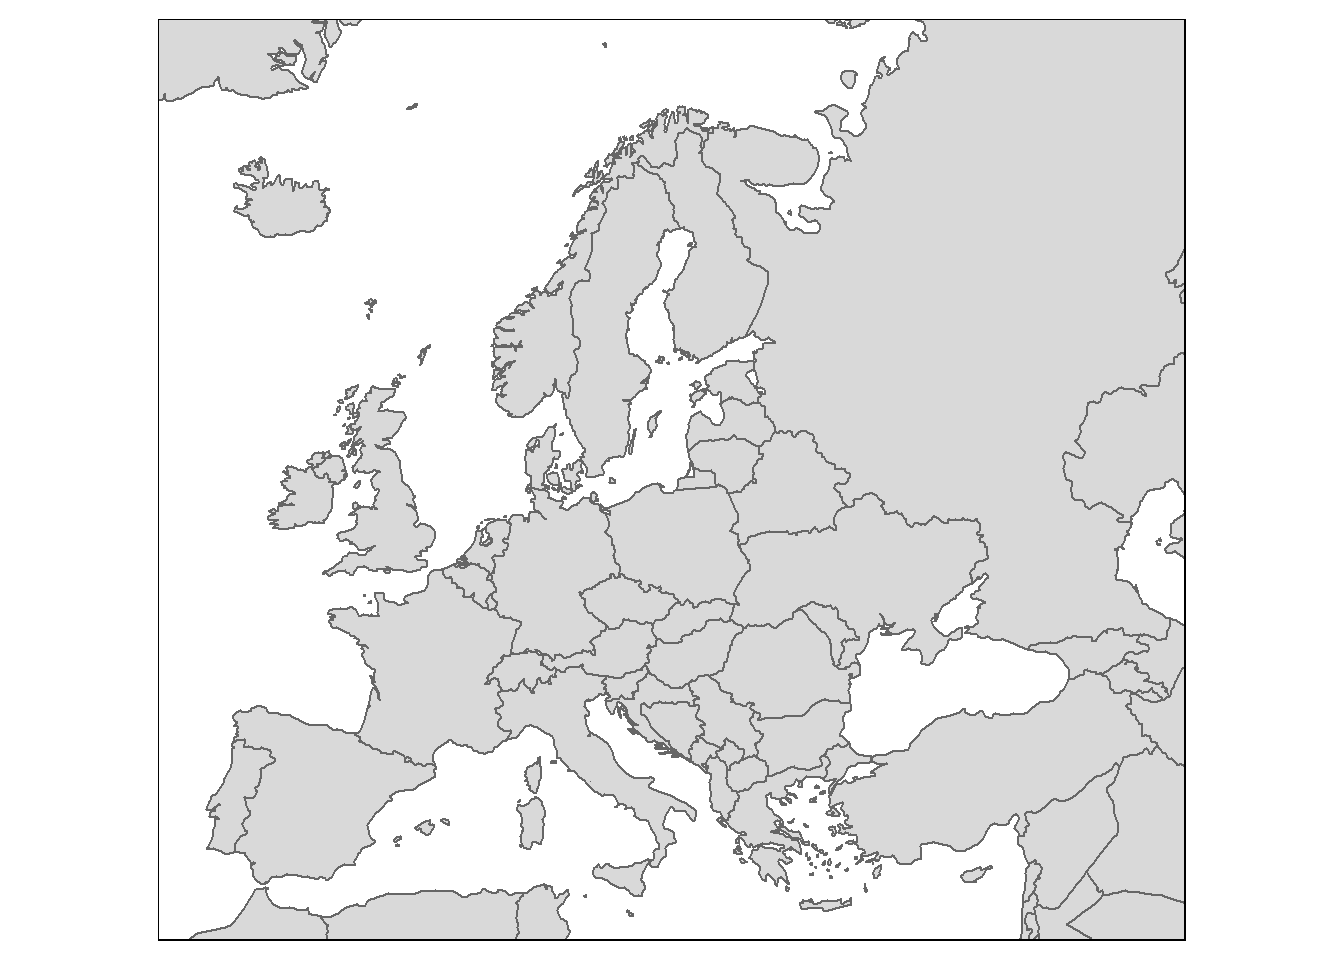
\includegraphics{bookdown-rquer_files/figure-latex/chunk-tmapeurope-1.pdf}

Alternativamente, con \texttt{ggmap} podríamos generar el mapa de una
localización específica del siguiente modo:

\begin{Shaded}
\begin{Highlighting}[]
\KeywordTok{library}\NormalTok{(ggmap)}
\CommentTok{#localizamos con longitud y latitud la zona que queremos}
\NormalTok{cat <-}\StringTok{ }\KeywordTok{c}\NormalTok{(}\DataTypeTok{lon =} \FloatTok{1.6430518}\NormalTok{, }\DataTypeTok{lat =} \FloatTok{41.6960344}\NormalTok{)}
\CommentTok{#generamos el mapa indicando la fuente (google) y el zoom que queremos}
\NormalTok{map <-}\StringTok{ }\KeywordTok{get_map}\NormalTok{(}\DataTypeTok{location =}\NormalTok{ cat, }\DataTypeTok{source =} \StringTok{"google"}\NormalTok{, }\DataTypeTok{zoom =} \DecValTok{8}\NormalTok{)}
\KeywordTok{ggmap}\NormalTok{(map)}
\end{Highlighting}
\end{Shaded}

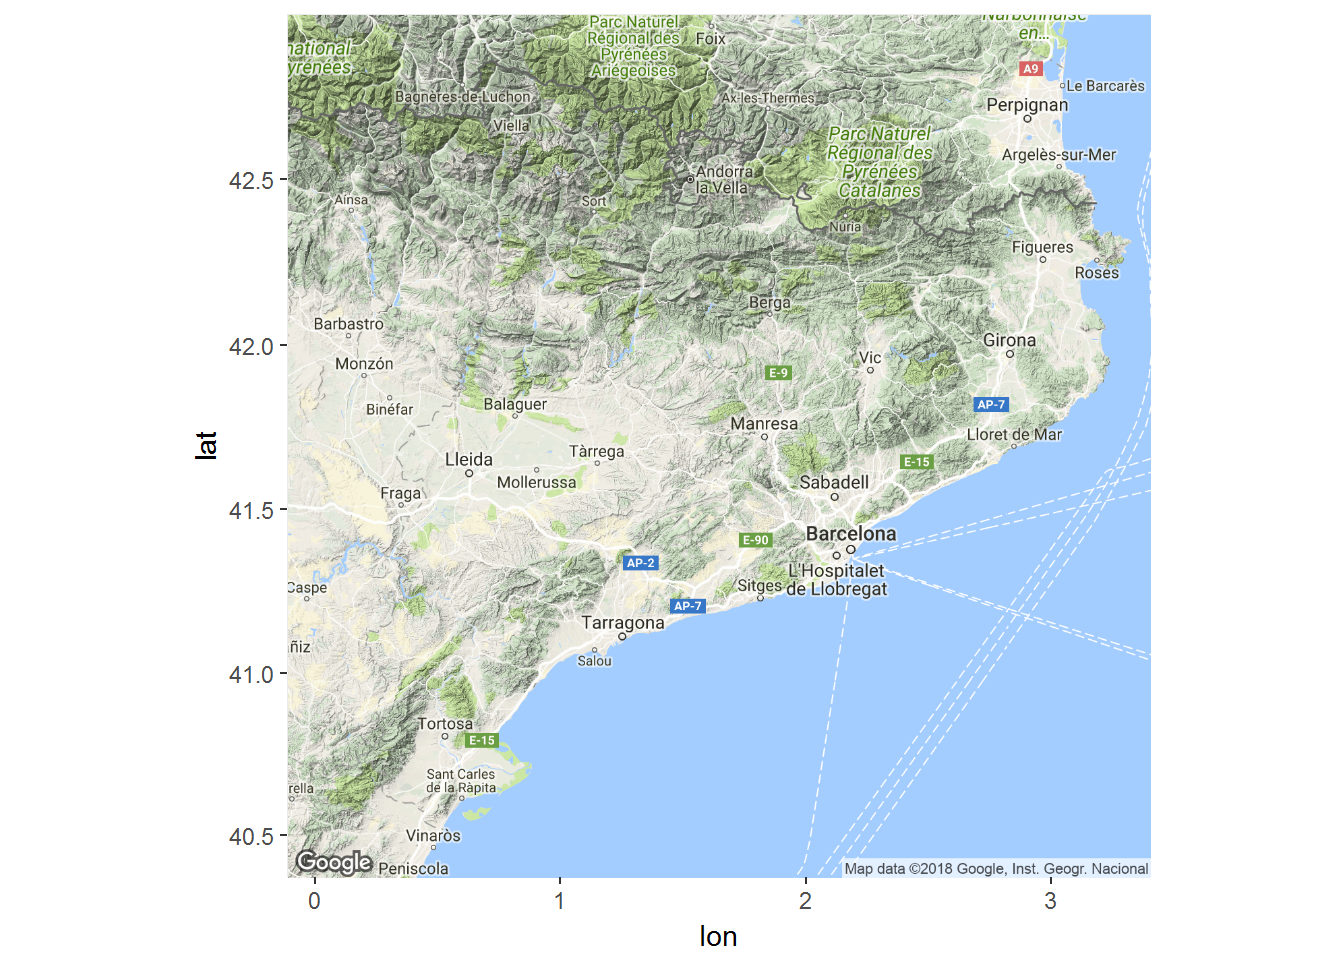
\includegraphics{bookdown-rquer_files/figure-latex/chunk-ggmap-1.pdf}

Si quisieramos otro tipo de representación (maptype) y color (por
ejemplo en blanco y negro) indicaríamos:

\begin{Shaded}
\begin{Highlighting}[]
\CommentTok{#el tipo de mapa de google puede ser “roadmap”, “terrain”, “satellite” o “hybrid”}
\NormalTok{map <-}\StringTok{ }\KeywordTok{get_map}\NormalTok{(}\DataTypeTok{location =}\NormalTok{ cat, }\DataTypeTok{source =} \StringTok{"google"}\NormalTok{, }\DataTypeTok{zoom =} \DecValTok{8}\NormalTok{, }\DataTypeTok{maptype =} \StringTok{"roadmap"}\NormalTok{, }\DataTypeTok{color =} \StringTok{"bw"}\NormalTok{)}
\KeywordTok{ggmap}\NormalTok{(map)}
\end{Highlighting}
\end{Shaded}

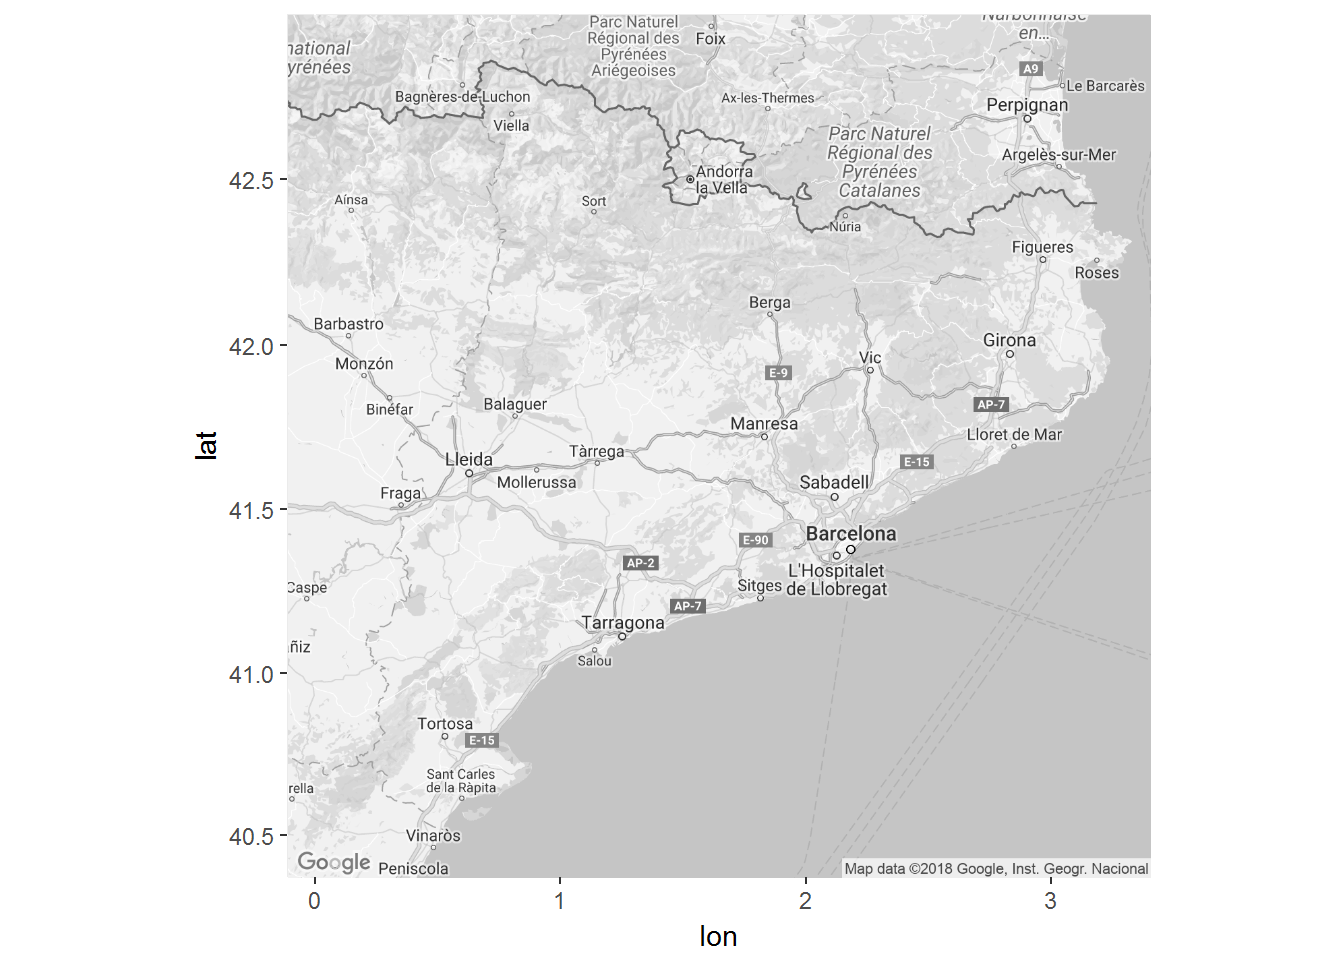
\includegraphics{bookdown-rquer_files/figure-latex/chunk-ggmapbw-1.pdf}

Si ahora quiero añadir un punto en el mapa (por ejemplo mi ciudad,
Barcelona):

\begin{Shaded}
\begin{Highlighting}[]
\CommentTok{#añado la long/lat de Barcelona}
\KeywordTok{ggmap}\NormalTok{(map) }\OperatorTok{+}\StringTok{ }\KeywordTok{geom_point}\NormalTok{ (}\KeywordTok{aes}\NormalTok{ (}\DataTypeTok{x =} \FloatTok{2.1734}\NormalTok{, }\DataTypeTok{y =} \FloatTok{41.3851}\NormalTok{),  }
                         
\CommentTok{#e indico la transparencia (alpha), color y tamaño del punto}
\DataTypeTok{alpha =} \FloatTok{.3}\NormalTok{, }\DataTypeTok{color =} \StringTok{"steelblue"}\NormalTok{, }\DataTypeTok{size =} \DecValTok{5}\NormalTok{)}
\end{Highlighting}
\end{Shaded}

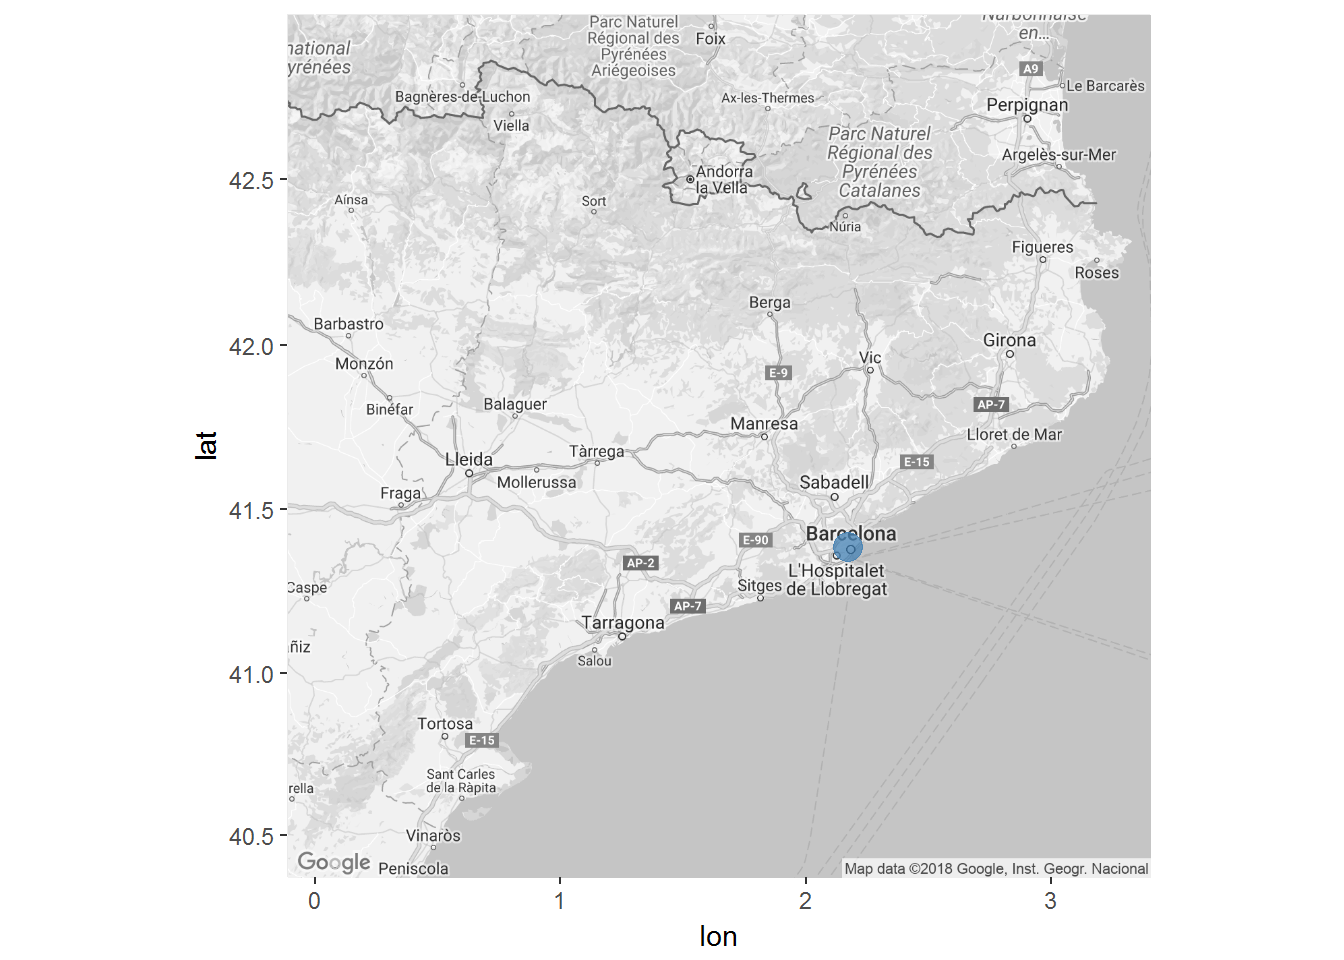
\includegraphics{bookdown-rquer_files/figure-latex/chunk-ggmapbcn-1.pdf}

Incluso puedo añadir datos al mapa; por ejemplo, los distritos de la
ciudad:

\begin{Shaded}
\begin{Highlighting}[]
\CommentTok{#primero encuentro las shapefiles de los distritos de Barcelona en datos abiertos:}
\CommentTok{#https://laura-an.carto.com/tables/shapefile_distrito_barcelona/public}
\CommentTok{#me las descargo en mi directorio de trabajo}

\CommentTok{#focalizo el mapa en Barcelona}
\NormalTok{bcn <-}\StringTok{ }\KeywordTok{c}\NormalTok{(}\DataTypeTok{lon =} \FloatTok{2.1734}\NormalTok{, }\DataTypeTok{lat =} \FloatTok{41.3851}\NormalTok{)}
\NormalTok{map <-}\StringTok{ }\KeywordTok{get_map}\NormalTok{(}\DataTypeTok{location =}\NormalTok{ bcn, }\DataTypeTok{source=}\StringTok{"google"}\NormalTok{, }\DataTypeTok{zoom =} \DecValTok{11}\NormalTok{, }\DataTypeTok{maptype =} \StringTok{"roadmap"}\NormalTok{, }\DataTypeTok{color =} \StringTok{"bw"}\NormalTok{)}

\CommentTok{#cargo el paquete rgdal para importar las shapefiles de los distritos al mapa}
\KeywordTok{library}\NormalTok{(rgdal)}
\NormalTok{shapefiles <-}\StringTok{ }\KeywordTok{readOGR}\NormalTok{(}\DataTypeTok{dsn =} \StringTok{"_bookdown_files/shapefile_distrito_barcelona.shp"}\NormalTok{,}
                    \DataTypeTok{layer =} \StringTok{"shapefile_distrito_barcelona"}\NormalTok{) }
\end{Highlighting}
\end{Shaded}

\begin{verbatim}
## OGR data source with driver: ESRI Shapefile 
## Source: "_bookdown_files/shapefile_distrito_barcelona.shp", layer: "shapefile_distrito_barcelona"
## with 10 features
## It has 12 fields
\end{verbatim}

\begin{Shaded}
\begin{Highlighting}[]
\CommentTok{#lo represento en el mapa:}
\KeywordTok{ggmap}\NormalTok{(map) }\OperatorTok{+}\StringTok{ }\KeywordTok{geom_polygon}\NormalTok{(}\KeywordTok{aes}\NormalTok{(}\DataTypeTok{x =}\NormalTok{ long, }\DataTypeTok{y =}\NormalTok{ lat, }\DataTypeTok{group=}\NormalTok{id), }
\DataTypeTok{data =}\NormalTok{ shapefiles, }\DataTypeTok{color =} \StringTok{"white"}\NormalTok{, }\DataTypeTok{fill =} \StringTok{"orange"}\NormalTok{, }
\DataTypeTok{alpha =} \FloatTok{.3}\NormalTok{, }\DataTypeTok{size =} \FloatTok{.2}\NormalTok{)}
\end{Highlighting}
\end{Shaded}

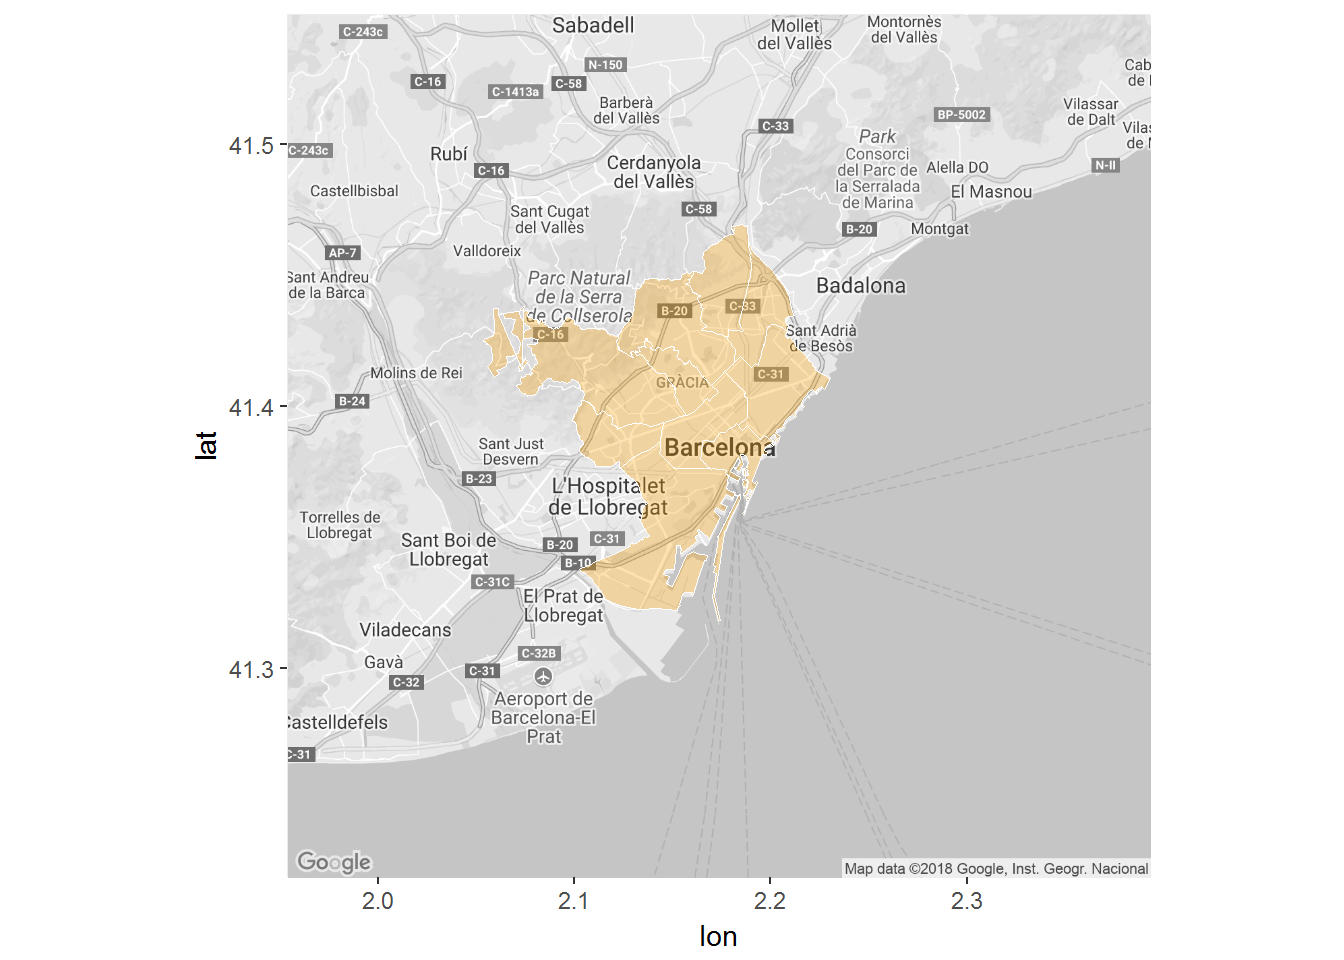
\includegraphics{bookdown-rquer_files/figure-latex/chunk-bcnshp-1.pdf}

\hypertarget{r-que-r}{%
\chapter{R que R}\label{r-que-r}}

He intentado mostrar en esta brevísima introducción a R, las
funcionalidades básicas de este lenguaje de Programación estadística y
algunas de las aplicaciones posibles. Esto ha sido sólo una muestra para
despertar el apetito. Uno de los aspectos más positivos de este lenguaje
es, precisamente, la activa comunidad de usuarios que existe a su
entorno, gracias a la cual es muy fácil obtener soporte para problemas
específicos y seguir aprendiendo mediante infinitud de recursos, muchos
de ellos gratuitos.

A continuación os dejo una lista de recursos para seguir aprendiendo R
que R.

\hypertarget{tutoriales}{%
\section{Tutoriales}\label{tutoriales}}

Algunos materiales interesantes para seguir aprendiendo son:

\begin{itemize}
\item
  El libro \href{https://r4ds.had.co.nz/}{R for Data Science} de
  \textbf{Hadley Wickham}, experto neozelandés que trabaja en RStudio.
  Toda una referencia actual en el desarrollo de este lenguage de
  programación y creador e integrador de gran cantidad de paquetes que
  facilitan todo el proceso analítico.
\item
  \href{https://www-bcf.usc.edu/\%7Egareth/ISL/}{An Introduction to
  Statistical Learning with Applications in R (ISLR)} de los profesores
  de Stanford \textbf{Trevor Hastie} y \textbf{Rob Tibshirani}. Mucho
  conocimiento transmitido de un modo muy cálido y relajado.
\item
  \href{http://varianceexplained.org/RData/}{Variance Explained} de
  \href{https://twitter.com/drob}{\textbf{David Robinson}} videos
  cortos, super claros y explicativos.
\item
  El libro \href{http://tidytextmining.com/intro.html}{Tidy Textmining},
  escrito por \href{https://juliasilge.com/}{\textbf{Julia Silge}} y
  David Robinson.
\item
  \href{https://www.r-bloggers.com}{R-bloggers}, blog curado por
  \textbf{Tal Galili}, Doctor de la Universidad de Tel Aviv. Enrorme
  repositorio de posts de miembros de de la comunidad de R a nivel
  mundial.
\item
  \href{https://www.twotorials.com/}{twotorials} de \textbf{Anthony
  Damico} una introducción muy ágil y divertida a R (videos de 2 minutos
  usando R en bruto ¡sin Rstudio!).
\item
  \href{http://www.datasciencecentral.com}{Data Science Central} de
  \textbf{Vincent Granville}.
\item
  \href{http://www.kdnuggets.com/}{KDnuggets} de \textbf{Gregory
  Piatetsky}.
\item
  \href{http://kirkborne.net/}{Kirk Borne} científico de datos principal
  en la consultora pionera BoozAllen.
\item
  \href{https://www.analyticsvidhya.com}{Analytics Vidhya} blog de un
  equipo muy activo de analistas de Bombay, liderados por \textbf{Kunal
  Jail} y que son además excelentes comunicadores y están siempre a la
  última de los avances en análisis de datos y Machine Learning,
  lenguajes de programación, etc. Como la gente de Rstudio y Datacamp,
  también publican útiles ``chuletas'' o
  \href{https://www.analyticsvidhya.com/blog/2017/02/top-28-cheat-sheets-for-machine-learning-data-science-probability-sql-big-data/}{Cheat
  Sheets} Para principiantes pero también para usuarios más avanzados.
\item
  \href{http://math.agrocampus-ouest.fr/infoglueDeliverLive/membres/Francois.Husson}{François
  Husson}, análisis de datos multivariantes y técnicas de clusterización
  con R.
\item
  Para trabajar con predicciones en series temporales es muy útil el
  trabajo del profesor \href{https://www.otexts.org/fpp}{Rob J Hyndman}
  de la Monash University, creador del paquete
  \href{http://robjhyndman.com/software/forecast/\%22}{Forecast}.
\end{itemize}

Otros recursos abiertos y gratuitos útiles son:

\begin{itemize}
\item
  Los excelentes materiales del curso
  \href{http://cm.dce.harvard.edu/2014/01/14328/publicationListing.shtml}{CSI
  E-109} del Harvard Distance Education, impartido por los porfesores de
  Harvard \_professors \textbf{Joe Blitzstein}, \textbf{Hanspeter
  Pfister} y \textbf{Verena Kaynig-Fittkau}.
\item
  Inventarios de recursos intersantes como
  \href{http://datasciencemasters.org}{Data Science Masters} de
  \textbf{Clare Corthell} de Summer.ai
\item
  \href{http://learnds.com/}{Learn Data Science} de \textbf{Nitin
  Borwankar}.
\item
  \href{https://www.kaggle.com}{Kaggle} Plataforma, red social de
  científicos de datos y entorno para competiciones de proyectos de
  minería de datos, aprendizaje automático y modelos predicitivos,
  creada por Anthony Goldbloom.
\end{itemize}

\href{https://www.datacamp.com}{Datacamp}, Coursera y Udacity, entre
otros ponen al alcance de todos el poder iniciarse en ciencia de datos y
R.

Finalmente, existen numerosos blogs personales de doctorandos,
\emph{practitioners} o usuarios apasionados de R que muestran modos de
analizar datos para casos específicos. También es sumamente útil
encontrar
\href{http://rmarkdown.rstudio.com/r_notebooks.html}{\textbf{notebooks}}
donde se conjugan scripts de código y explicaciones de los mismos.

\hypertarget{obtener-ayuda}{%
\section{Obtener ayuda}\label{obtener-ayuda}}

Ya vimos que podemos obtener ayuda sobre una función o un objeto usando
\texttt{?} o \texttt{help()}. Para acceder a la ayuda general en R
podemos escribir \texttt{help.start()} o usar la pestaña \texttt{help}
(si estamos en el entorno de Rstudio). También podemos usar
\texttt{vignette()} para visualizar una descripción detallada de un
paquete, de para qué sirve y de cómo usarlo.

Cuando al ejecutar comandos nos aparece un error (mensaje de texto en
rojo en la consola de R), es importante leerlo para aprender de él
(¡como en la vida!).

Otra gran opción que tenemos para resolver errores es buscar en la web
de preguntas y respuestas
\href{https://stackoverflow.com}{\textbf{stackoverflow}}
\url{https://stackoverflow.com}. Si simplemente copiamos y pegamos el
error que nos aparece en R en Google, es muy probable que nos dirija a
stackoverflow. Y es muy probable también que en uno de sus foros alguien
haya solucionado ya el problema que buscamos u otro similar que nos
ayude a entender. De igual modo podemos contribuir allí y aclarar dudas
a otros. Estos foros de preguntas y respuestas son, por lo general, una
enorme fuente de aprendizaje y una inyección de optimismo en la
humanidad.

\hypertarget{sumario}{%
\chapter{Sumario}\label{sumario}}

Espero que este libro te haya servido para iniciarte en el análisis de
datos con R y que hayas podido entrever sus grandes posibilidades
analíticas.

No hemos hablado de otras muchas técnicas estadísticas posibles en R,
desde opciones gráficas (incluso interactivas) a opciones para procesar
contenidos textuales que en R pueden implementarse mediante paquetes
como \texttt{tm}, \texttt{OpenNLP} o \texttt{tidytext} u otros,
algoritmos de Aprendizaje automático, mediante paquetes como
\texttt{e1071}, \texttt{randomForest} o \texttt{Caret}, entre muchos,
muchos otros. Las aplicaciones son infinitas. Nos queda todavía mucho
que aprender.

¿Te enganchó?

A seguir pues, \textbf{¡R que R!}

¡Muchas gracias!

Enric Escorsa O'Callaghan

\bibliography{book.bib,packages.bib}


\end{document}
